\chapter{Peculiarities of undulator imaginary source distribution}
\label{Chapter:Undulator radiation imaginary source peculiarities}

    \rr{to be improved, first two paragraphs sound too ragged}
    
    Undulator radiation has been extensively studied and utilized at synchrotron radiation sources for decades. Needless to say, it has been described in great detail both theoretically~\cite{theoretical_reference} and experimentally~\cite{experimental_reference}. However, only recently has an analytical expression for the virtual source distribution for radiation from a single electron been provided~\cite{geloni_statistical_2006, geloni_fourier_2007}. This kind of distribution has a direct physical meaning and can be reproduced using a 1:1 focusing system. The importance of understanding the single electron distribution at the source location cannot be overstated. First of all, it is crucial for examining the transverse coherence properties of synchrotron radiation. In fact, the cross-spectral density of the radiation is expressed through the single electron distribution~\cite{geloni_transverse_2008}.
    
    Moreover, modern synchrotrons employing multi-bend achromat (MBA) magnetic structures~\cite{mba_reference} and reaching the X-ray wavelength range operate in a regime where the single electron beam size and divergence dominate over the electron beam size and divergence. The authors of~\cite{geloni_fourier_2007} noted that although the undulator radiation source distribution is “laser-like,” there are peculiarities at both ends of the source distribution for frequencies around undulator resonance at the odd harmonics. This suggests that there is more to study in this area.
    
    In this chapter, I aim to study the undulator radiation imaginary source in greater detail than has previously been presented. I will start with a general expression for synchrotron radiation, beginning with the inhomogeneous electromagnetic wave equation. Assuming that the particles emitting the radiation are ultra-relativistic and using the slowly varying envelope approximation (SVEA), I will derive a paraxial wave equation, which is commonly used to characterize synchrotron radiation. Subsequently, I will provide an analytical solution for undulator radiation under the resonance approximation at any given position along an optical line. This expression assumes three approximations: the paraxial approximation, the SVEA, and the resonance approximation specific to the undulator case. The resonance approximation implies a sufficiently large number of undulator periods and considers the radiation around the odd harmonic resonance frequencies.
    
    To avoid the resonance approximation, I will analyze the undulator radiation imaginary source distribution in detail using numerical wavefront propagation methods. This analysis will highlight the features that appear at both ends of the undulator’s imaginary source, as initially noted in~\cite{geloni_fourier_2007}. The apparent width of this feature reveals a finer structure of undulator radiation than is typically associated with the usual diffraction size given by $\sqrt{L_w \lambdabar}$, where $L_w$ is the undulator length.
    
    To investigate this further, I will examine the source behavior by reducing the number of undulator periods, thus extending beyond the resonance approximation~\footnote{In this chapter, I use two closely related terms: the \textit{resonance approximation} and radiation \textit{in resonance} or \textit{resonance condition}. The first term refers to the derivation of the undulator radiation analytical expression for the far zone, implying a large number of undulator periods, an observation angle confined to the central cone of undulator radiation, and a radiation frequency around the \textit{resonance condition}. The \textit{resonance condition} indicates that undulator radiation is considered at its resonance frequency of odd harmonics.}. This reduction results in a ‘wiggling’ effect of the source, replicating the actual electron path in the undulator. Additionally, I will explore the source distribution at the non-resonance frequency. As a result, this chapter will provide an overview of the nature of these peculiarities and propose two experiments at synchrotron radiation facilities to reveal them.
    
\section{Radiation from a charged particle in electromagnetic fields}

    In this section, I derive the paraxial wave equation for synchrotron radiation. The derivations in this section are based on~\cite{geloni_paraxial_2005}. Starting with the Helmholtz wave equation from Chapter~\ref{chapter:introduction}:
    \begin{align}
        c^2 \nabla^2 \vec{\bar{E}} + \omega^2 \vec{\bar{E}} = 4 \pi c^2 \vec{\nabla} \bar{\rho} - 4 \pi i \omega \vec{\bar{j}},
        \label{Eq}
    \end{align}
    I can simplify this equation using the slowly varying envelope approximation (SVEA), where I extract the highly oscillatory component in the propagation direction from the intensity. Introducing a fixed Cartesian reference system $(x,y,z)$, where $z$ is the optical axis:
    \begin{align}
        \bar{E} = \tilde{E}e^{i \omega z / c},
    \end{align}
    which implies that $\tilde{E}$ varies slowly on the scale of the wavelength $\lambda = 2 \pi c / \omega$. This factorization into the slow and fast varying functions helps to further reduce the wave equation by substituting it into the expression under Eq.~\ref{Eq}:
    \begin{align}
        c^2 e^{i \omega z / c} \bigg( \nabla^2 + \frac{2 i \omega}{c} \frac{\partial }{\partial z} \bigg)\vec{\tilde{E}} = 4 \pi c^2 \vec{\nabla} \bar{\rho} - 4 \pi i \omega \vec{\bar{j}}.
        \label{Eq}
    \end{align}
    Next, I write this equation for a specific source: a single electron moving along a curvilinear abscissa $s$ in a magnetic field. The latter means that its velocity $v = |\vec{v}(t)|$ is constant. Thus, the curvilinear abscissa can be expressed as $s = vt$.
    
    I consider radiation from a single electron, so the charge density and current density can be expressed mathematically via Dirac delta functions:
    \begin{align}
        \rho(\vec{r}, t) = -e\delta\big(\vec{r} - \vec{r}'(t)\big)  
        \label{Eq:rho}
    \end{align}
    and
    \begin{align}
        \vec{j}(\vec{r}, t) = -e\vec{v}(t)\delta\big(\vec{r} - \vec{r}'(t)\big),
        \label{Eq:j}
    \end{align}
    where $\vec{r}'(t)$ and $\vec{v}(t)$ are the electron's position and velocity in a given reference frame. The particle trajectory in the magnetic field should be determined separately using dynamic equations, which are assumed here to be given \textit{a priori}.
    
    I rewrite $\delta\big(\vec{r} - \vec{r}'(t)\big)$ as $\delta\big(\vec{r} - \vec{r}'(t)\big) = \delta \big(\vec{r}_{\perp} - \vec{r}'_{\perp}(t)\big)\delta\big(z - z'(t)\big)$ separating longitudinal and transverse dimensions. And then I can rewrite it as the following:
    \begin{align}
        \delta\big(z - z'(t)\big) = \frac{1}{v_z(z)}\delta\big(t - t(z) \big),
    \end{align}
    using the well known property of the delta function:
    \begin{align}
        \delta\big(f(x)\big) = \sum_i \frac{\delta(x - x_i)}{f'(x_i)}, 
    \end{align}
    where I denoted $\delta\big(z - z'(t)\big)$ as $\delta \big[f(t)\big]$, for any fixed value of $z$. There is the only zero for the function $z - z'(t)$ at the $t$ value that is indicated by $t(z)$. Also $|f'(t(z))| = v_z(z(t))$.
    
    So, remembering that $s(z) = u t(z)$ I rewrite $\rho$ and $\vec{j}$ from Eqs.~\ref{Eq:rho} and~\ref{Eq:j} as the following:
    \begin{align}
        \rho(\vec{r}_{\perp}, z, t) = - \frac{e}{v_z(z)}\big(\vec{r}_{\perp} - \vec{r}'_{\perp}(t)\big)\delta\bigg(\frac{s(z)}{v} - t\bigg)
    \end{align}
    and 
    \begin{align}
        \vec{j}(\vec{r}_{\perp}, z, t) = -\frac{e}{v_z(z)} \vec{v}(z)\delta \big(\vec{r}_{\perp} - \vec{r}'_{\perp}(t)\big)\delta\bigg(\frac{s(z)}{v} - t\bigg).
    \end{align}
    Then performed Fourier transform I obtain:
    \begin{align}
        \bar{\rho}(\vec{r}_{\perp}, z, \omega) = - \frac{e}{v_z(z)}\delta\big(\vec{r}_{\perp} - \vec{r}'_{\perp}(z)\big)e^{i\omega s(z)/ v}
        \label{Eq:rho_w_domain}
    \end{align}
    and
    \begin{align}
        \vec{\bar{j}}(\vec{r}_{\perp}, z, \omega) = - \frac{e}{v_z(z)} \vec{v}(z)\delta\big(\vec{r}_{\perp} - \vec{r}'_{\perp}(z)\big)e^{i\omega s(z)/ v}.
        \label{Eq:j_w_domain}
    \end{align}
    And now I rewrite Eq.~\ref{Eq:wave_eq_SVEA} substituting Eqs.~\ref{Eq:rho_w_domain} and~\ref{Eq:j_w_domain} in it I obtain:
    \begin{align}
        \bigg( \nabla^2 + \frac{2 i \omega}{c} \frac{\partial }{\partial z} \bigg) \vec{\tilde{E}} = \frac{4 \pi e}{v_z(z)} \exp{\bigg[ i\omega \bigg(\frac{s(z)}{v} - \frac{z}{c} \bigg)\bigg] \bigg[i \frac{\omega}{c^2} \vec{v}(z) - \vec{\nabla}\bigg]\delta\big(\vec{r}_{\perp} - \vec{r}'_{\perp}(z)\big)}.
        \label{Eq:nonhomogeneous_wave_eq_SVEA_mod}
    \end{align}
    This equation is still very general, but before reducing it to the paraxial form, I wish to discuss the influence of the exponential factor $\exp{[ i\omega (s(z)/v - z/c )]}$ on the final solution of the integral form~\cite{ref}~(introduced in Chapter 1 with the Green's function). Under the integral, this phase factor will cause the integrand to be highly oscillatory, which will generally cause the integral's contribution to vanish unless $\omega (s(z)/v - z/c ) \sim 1$. The length at which this happens is referred to as the formation length ($L_f$) of radiation at the given frequency $\omega$.

    If I take the velocity ($v$) of the particle to be of the order of the speed of light but noticeably smaller, I can find that $L_f \sim \lambda$. However, in the ultra-relativistic case when $v$ is very close to the speed of light ($\gamma^2 \gg 1$), it happens that $s(z)/v$ and $z/c$ compensate each other, resulting in $L_f$ being significantly larger than $\lambda$. The exact expression for $L_f$ in this case largely depends on the considered magnetic configuration, which I address later in this chapter using the example of undulator radiation.

    In this thesis, I consider the case of ultra-relativistic particles, i.e., $\gamma^2 \gg 1$. This assumption provides significant simplification for the wave equation in Eq.~\ref{Eq} and has two general practical results: as mentioned, the formation length will be much longer than the wavelength ($L_f \gg \lambda$), and almost all the power of the radiation will be concentrated in the central cone of order $1/\gamma$, which is a result of the "Lorentz boost" or eponymous transformation. The latter is very valuable as small angles always ensure that the paraxial approximation is \textit{automatically} fulfilled for the case of radiation from ultra-relativistic particles.   

    As mentioned, $\vec{\tilde{E}}$ does not vary much along the propagation axis $z$ on the scale of $\lambda$, which can be mathematically expressed as $|\partial \tilde{E}_{x, y}| \ll (\omega/c)|\tilde{E}_{x, y}|$. Therefore, the second derivative with respect to $z$ in the nabla operator will be much smaller than the first derivative present in the expression. This allows for a significant simplification of Eq.~\ref{Eq} by applying the paraxial approximation:
    \begin{align}
        \bigg( \nabla^2_\perp + \frac{2 i \omega}{c} \frac{\partial }{\partial z} \bigg) \vec{\tilde{E}}_\perp = \frac{4 \pi e}{c} \exp{\bigg[ i\omega \bigg(\frac{s(z)}{v} - \frac{z}{c} \bigg)\bigg] \bigg[i \frac{\omega}{c^2} \vec{v}_\perp(z) - \vec{\nabla}\bigg]\delta\big(\vec{r}_{\perp} - \vec{r}'_{\perp}(z)\big)}
        \label{Eq:nonhomogeneous_paraxial_wave_eq}
    \end{align}
    Writing this partial differential equation, I notice that it has been transformed to the parabolic type.
    
\subsection{Solution of the paraxial wave equation in a free space}
    The solution for Eq.~\ref{Eq} is relatively easy to find using the Green's function approach. A Green's function should satisfy the following equation:
    \begin{align}
        \bigg( \nabla^2 + \frac{2 i \omega}{c} \frac{\partial }{\partial z} \bigg) G(z_0 - z; \vec{r}_{\perp 0} - \vec{r}_{\perp}) = \delta(\vec{r}_{\perp 0} - \vec{r}'_{\perp})\delta(z_0 - z), 
        \label{Eq:Green_func_delta}
    \end{align}
    that effectively describes radiation from a point source. In the case of free space, the solution for this equation is well known and can be written as follows:
    \begin{align}
        G(z_0 - z; \vec{r}_{\perp 0} - \vec{r}_{\perp}) = -\frac{1}{4 \pi (z_0 - z')} \exp{\bigg[ i \omega \frac{|\vec{r}_{\perp 0} - \vec{r}'_{\perp}|^2}{2c(z_0 - z')}\bigg]}.
    \end{align}
    where, as usual, coordinates with primes correspond to the source location and those with $*_0$ refer to the observer location.
    
    One can express the solution of the non-homogeneous Eq.~\ref{Eq} via the Green's function $G(z_0 - z; \vec{r}_{\perp_0} - \vec{r}_{\perp})$ at the point $\vec{r}_{\perp_0}$, $z_0$ as an integral over $z'$ and $\vec{r}'$ under the right-hand side expression $f(z; \vec{r}'_{\perp})$ of the non-homogeneous equation:
    \begin{align}
        \vec{\tilde{E}}(\vec{r}_{\perp 0}, z_0) = \int_{-\infty}^{\infty} G(z_0 - z', \vec{r}_{\perp 0} - \vec{r}'_{\perp}) f(z', \vec{r}'_{\perp})d\vec{r}'_{\perp}dz'
        \label{Eq:nonhomogeneous_paraxial_wave_eq_solution_Green_function}
    \end{align}
    At this point, it is worth noting that this approach is very powerful for more general cases, such as a "bounded" case, e.g., a waveguide. This means that the solution of a non-homogeneous partial differential equation with boundary conditions can be written using the same integral Eq.\ref{Eq}, but with an appropriate Green's function. This Green's function should be found using Eq.\ref{Eq} with the imposed boundary conditions.
    
    Now I can explicitly write Eq.~\ref{Eq:nonhomogeneous_paraxial_wave_eq_solution_Green_function} with the right hand side substituted into the integral:
    \begin{align}
        \vec{\tilde{E}}_{\perp}(\vec{r}_{\perp 0}, z_0, \omega) = 
        \frac{e}{c} \int_{-\infty}^{\infty} dz' \frac{1}{z_0 - z'} 
        \int_{\mathbb{R}^2} d\vec{r}'_{\perp} \bigg[i \frac{\omega}{c^2} \vec{v}_{\perp}(z) - \vec{\nabla}_{\perp}\bigg]
        \delta\big(\vec{r}'_{\perp} - \vec{r}'_{\perp}(z)\big) \times
        \cr \exp{\bigg[i\omega \bigg(\cfrac{|\vec{r}_{\perp_0} - \vec{r}'_{\perp}|^2}{2c(z_0 - z')} +  \cfrac{s(z')}{v} - \frac{z'}{c} \bigg)\bigg]},
    \end{align}
    and then taking the integral over the transverse direction I obtain:
    \begin{align}
        \vec{\tilde{E}}_{\perp}(\vec{r}_{\perp 0}, z_0, \omega) = - \cfrac{i \omega e}{c^2}\int_{-\infty}^{\infty} dz' \frac{1}{z_0 - z'}
        \bigg[\bigg(\frac{v_x(z')}{c} - \cfrac{x_0 - x'(z')}{z_0 - z'}\bigg)\vec{e}_x + \bigg(\frac{v_y(z')}{c} - \cfrac{y_0 - y'(z')}{z_0 - z'}\bigg)\vec{e}_y\bigg] \times
        \cr \exp{\bigg[i\omega \bigg(\cfrac{(x_0 - x'(z'))^2 + (y_0 - y'(z'))^2}{2c(z_0 - z')} +  \cfrac{s(z')}{v} - \frac{z'}{c} \bigg)\bigg]}.
        \label{Eq:funal_Eq_for_SR}
    \end{align}
    This integral can now be directly used in the calculations of synchrotron radiation once the trajectory and velocity of an electron are known.

    The exact same result can be obtained using a Green’s function for the Helmholtz equation. Mathematically, there is no difference between applying the paraxial approximation at the stage of deriving the wave equation or at the stage of solving it. This result has been demonstrated in~\cite{geloni_paraxial_2005}. Moreover, it is clear from the section that the paraxial approximation can always be applied to Maxwell’s equations in the case of ultra-relativistic particles, as almost all the power of the radiation is concentrated in a narrow cone of $1/\gamma$. This approximation is not imposed artificially, as it is in some optical scenarios.

    Another point to mention is that traditionally, radiation from a charged particle is derived using the Liénard-Wiechert potential in the time domain. This is another way of approaching the problem but is completely equivalent to the approach presented here. This question is more extensively described in~\cite{geloni_paraxial_2005}.
    
    In conclusion, the integral in Eq.~\ref{Eq:funal_Eq_for_SR} can now be directly used in the calculations of synchrotron radiation once the trajectory and velocity of an electron are known.

    
\section{Undulator source studies}
    In this study, I consider the simple case of a planar undulator. I will analyze undulator radiation numerically, as any analytical approach for determining the field distribution from an undulator would inevitably require significant simplifications. These simplifications generally assume the device consists of many periods and is restricted to frequencies around the resonance condition. The primary assumption is the resonance approximation, which implies that all periods contribute constructively to the radiation field. This assumption aids in deriving the well-known field distribution in the far field zone. However, it also neglects many terms that are crucial to the effects I study in this chapter. Therefore, I will utilize numerical simulations to study undulator radiation. These simulations will be based on the general integral presented in the previous section or the integral derived from the Fourier transform of the Liénard-Wiechert potential \cite{chubar_accurate_1998, tanaka_spectra_2001, tomin_synchrotron_2019}. Before proceeding with numerical simulations, I will provide an analytical expression for the source distribution of undulator radiation. 

\subsection{Analytical expression for the undulator radiation field}
    In this section, I present the well-known expression for undulator radiation, using the derivation from~\cite{geloni_fourier_2007}:
    \begin{align}
        \vec{\tilde{E}}_{\perp}(\vec{r}_{\perp 0}, z_0, \omega) = - \cfrac{K \omega e L_w}{2 c^2 z_0 \gamma} A_{JJ} \textup{exp}{\bigg[\cfrac{i\omega z_0}{2 c}\theta^2 \bigg]} \textup{sinc}{\bigg[\cfrac{\omega L_w \theta^2}{4 c} \bigg]}, 
        \label{Eq:und_field_far}
    \end{align}
    where $L_w = \lambda_w N_w$ is the undulator length, $N_w$ is the number of undulator periods and $\lambda_w$ is the undulator length, $A_{JJ} = J_0(\zeta) - J_1(\zeta)$ where $\zeta = K^2 / (4 + 2 K^2)$ and $J_n$ is the $n$-th order Bessel function of the first kind. $K = e B \lambda_w/ 2 \pi m_e c$ is the undulator (deflection) parameter, where $m_e$ is the electron mass and $B$ is the maximum magnetic field in the undulator along the $z$-axis. Also angle $\vec{\theta}$ is the observation angle in the far zone that is equal to $\vec{r}_{\perp_0}/z$. 

    This expression describes the undulator field distribution in the far zone at the distance $z_0$ from the center of the undulator. Using the field propagator from~\cite{geloni_fourier_2007} or the one derived in Chapter~\ref{chapter:introduction}\footnote{They are equivalent in the paraxial approximation.}, I can now back propagate the field to the virtual source position $z_0 = 0$, which is located in the middle of the undulator:
    \begin{align}
        \tilde{E}_{\perp}(\vec{r}_{\perp 0}, 0, \omega) = i \cfrac{K \omega e}{2 c^2 \gamma} A_{JJ} \bigg[\pi - 2\textup{Si}\big(\cfrac{\omega \vec{r}_{\perp 0}}{L_w c}\big) \bigg]
        \label{Eq:und_field_source}
    \end{align}
    Actually, it is quite natural to define the source location of the undulator radiation at the very center of the undulator, where the phase distribution is flat. This choice of location seems logical from different points of view: the symmetry of the source radiation distribution with respect to the plane that perpendicularly crosses the center of the undulator to the optical axis, and the plane phase front, i.e., flat phase distribution. The first property is useful for adjusting the magnetic lattice, as it has a plane of symmetry, and the second one is essential for user experiments where focusing with a flat phase front is important for imaging techniques.
    
    Knowing this field distribution, I can obtain the distribution at an arbitrary observation position $z_0$ again using the free space propagator, and write it as follows~\cite{geloni_fourier_2007}:    
    \begin{align}
        \vec{\tilde{E}}_{\perp}(\vec{r}_{\perp 0}, z_0, \omega) = \cfrac{K \omega e A_{JJ}}{2 c^2 \gamma} \bigg[\textup{Ei}\bigg(\cfrac{i \omega r^2_{\perp}}{2z_0 c - L_w c}\bigg) - \textup{Ei}\bigg(\cfrac{i \omega r^2_{\perp}}{2z_0 c - L_w c}\bigg) \bigg],
    \end{align}
    where $\textup{Ei}(\cdot)$ indicates the exponential integral function. As noted in~\cite{geloni_fourier_2007}, the field at the points $z_0 = L_w/2$ and $r_{\perp} = 0$ is singular. The appearance of this mathematical singularity is related to the use of the resonance approximation. To the best of my knowledge, this passage has seemingly not drawn much attention, either theoretically or from an experimental point of view. In this thesis, I will study this peculiarity in more detail and, as a result, propose two methods for measuring it.
    
\subsection{Source peculiarities or Wigner function stretching at the source}
\rr{show Wigner function distribution and marginal distributions.} 

    The apparent singularity at both ends of the imaginary source of single electron undulator radiation can be studied numerically. However, a qualitative explanation can be viewed from the perspective of a Wigner function distribution in the transverse dimension of the synchrotron radiation~\cite{bazarov_synchrotron_2012}. In Fig.\ref{Fig:Lw2_wig}, I depict the Wigner function distribution at the center of the device (sub-figure framed in green). This distribution resembles a "cross." The marginal distributions onto the horizontal and vertical axes of the Wigner function will result in intensity distributions in the corresponding domains: real and inverse space, which in this case correspond to the coordinate and angular distribution of the source. In Fig.\ref{Fig:middle_scan}, I present the marginal distribution in the real space domain at the center of the undulator source along with its phase distribution. 
    \begin{figure*}[h!]
        \centering
        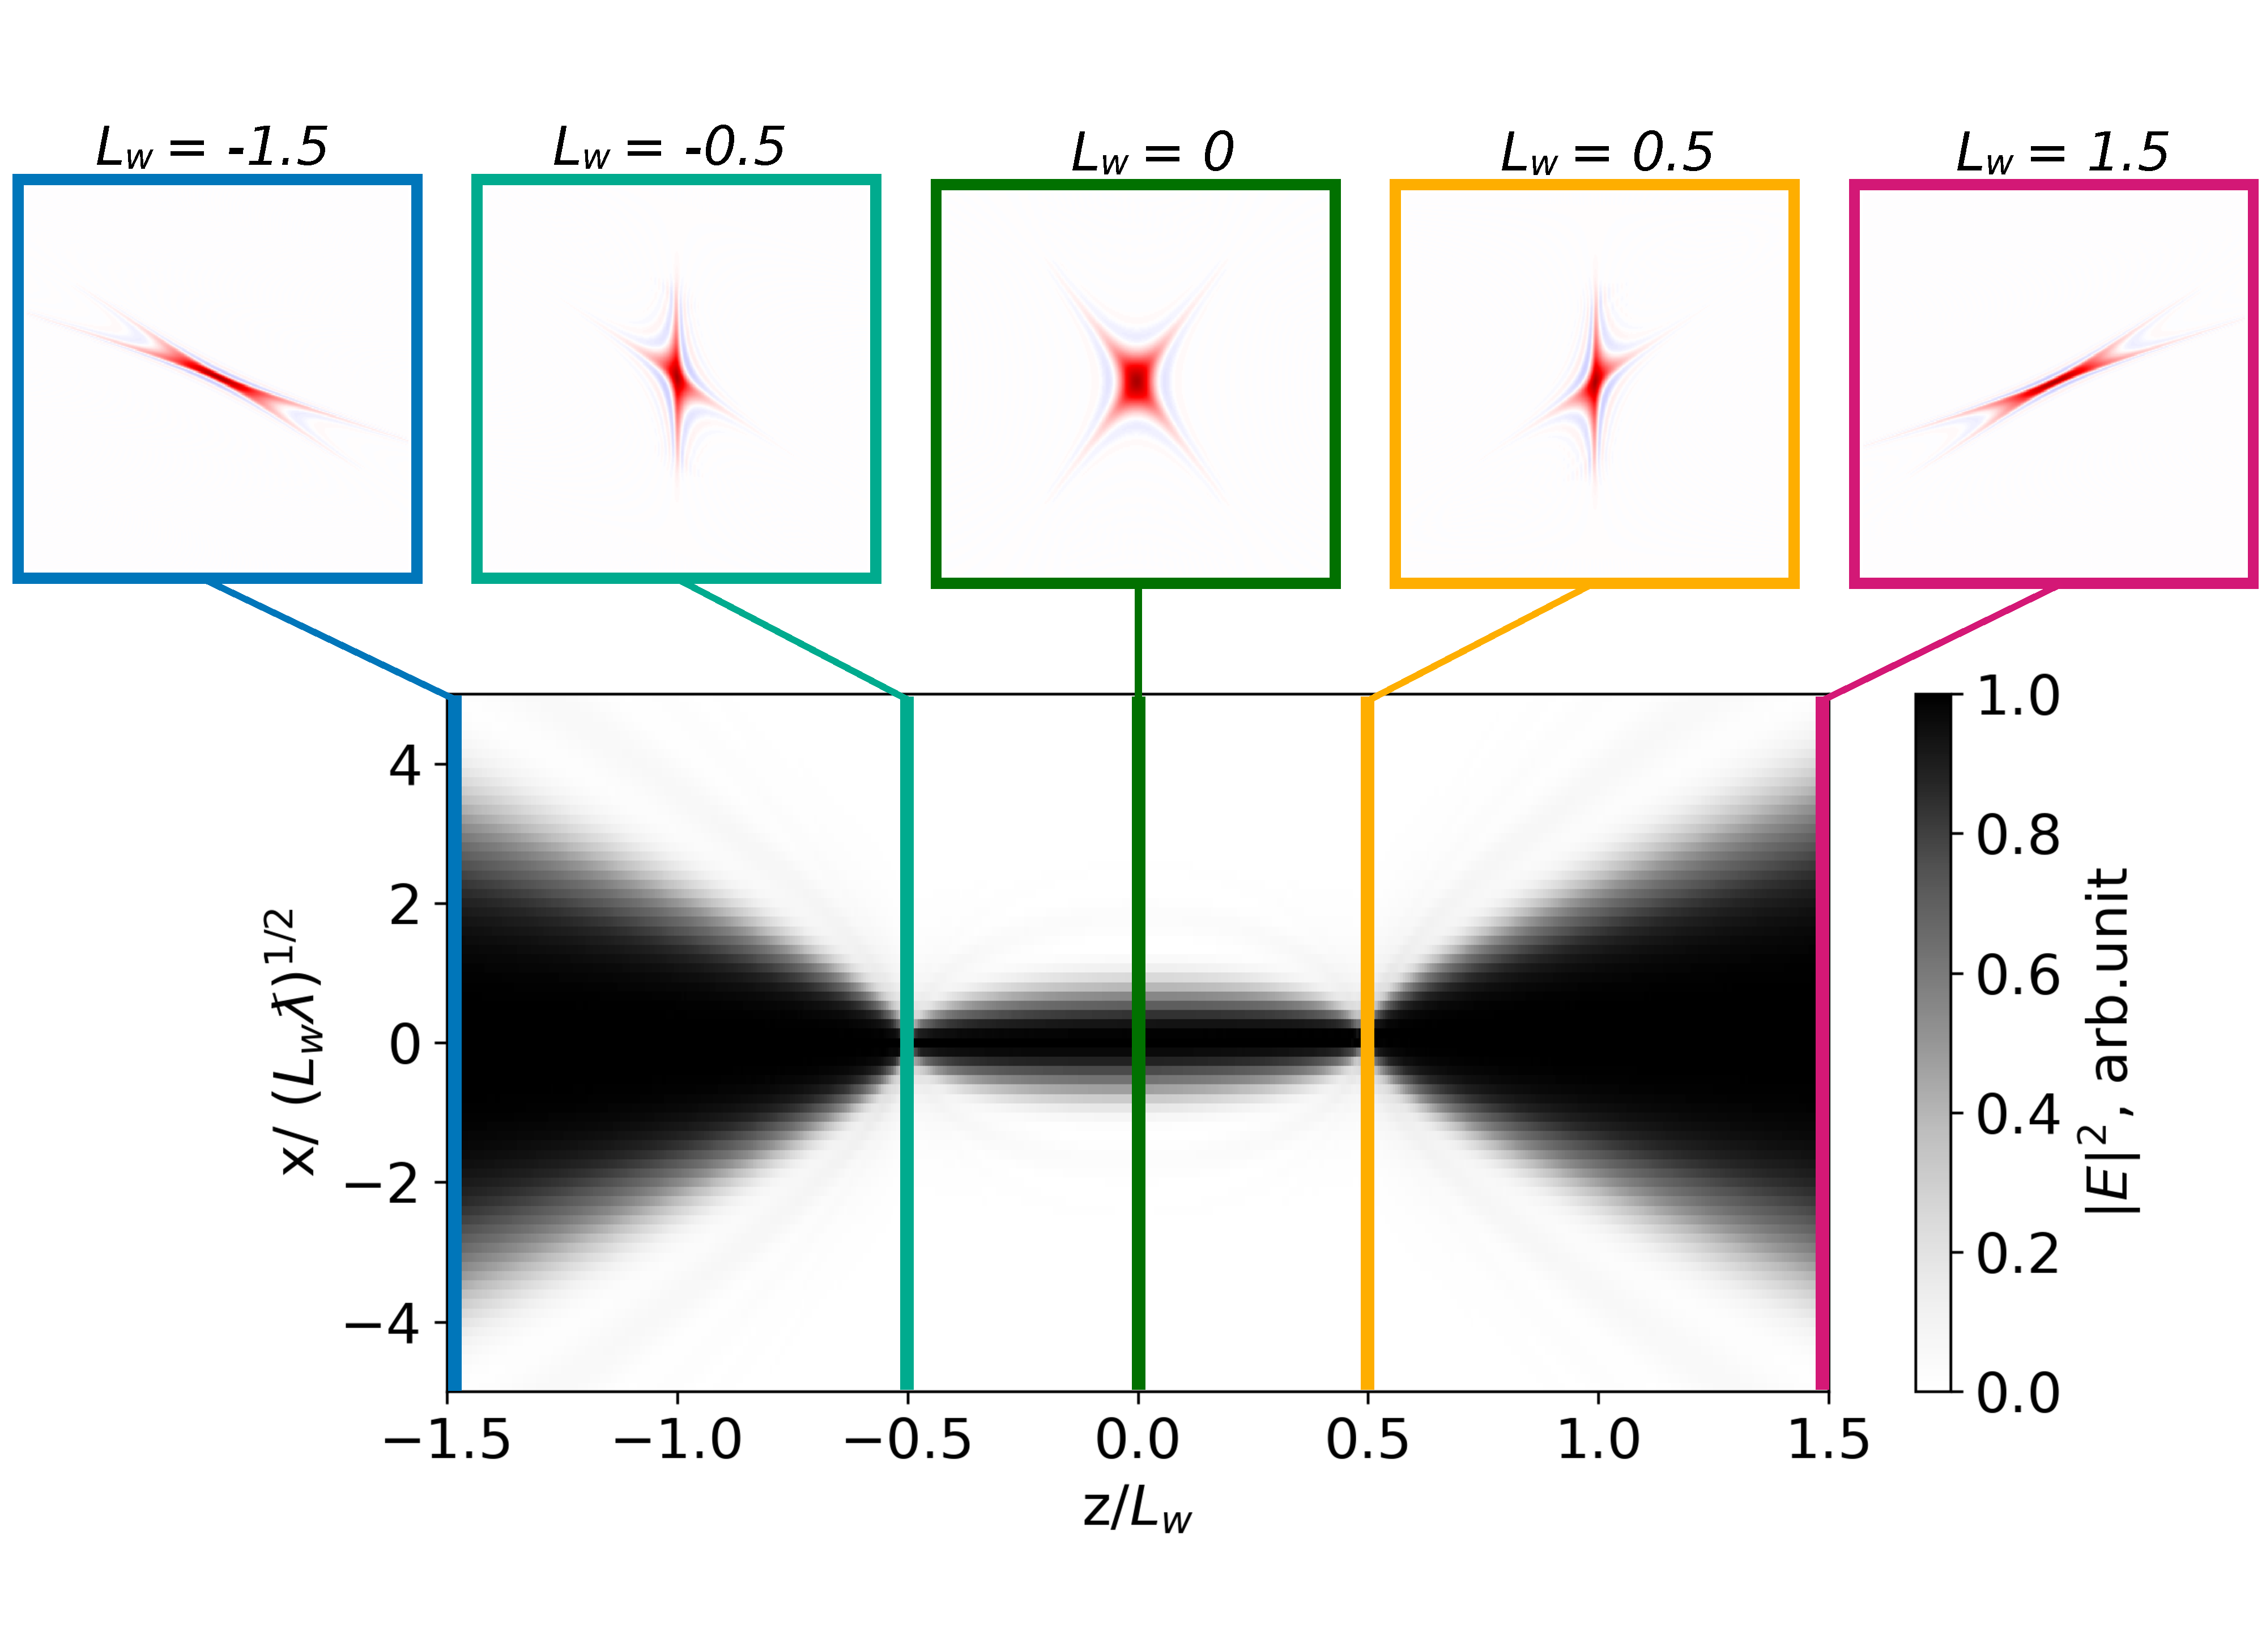
\includegraphics[width=0.9\linewidth]{content/images/Synchrotron_Radiation/Lw2_wig.pdf}
        \captionsetup{justification=centering}
        \caption{Source intensity distribution along an undulator versus the x-transverse dimension. Both axes are normalized to the natural dimensions of the system: undulator length and undulator radiation diffraction size. The intensity value along the slice over the vertical axis is normalized by the maximum of its intensity. At the top of the plot, I present Wigner function distributions at different positions along the device.}
        \label{Fig:Lw2_wig}
    \end{figure*}
    \begin{figure*}[h!]
        \centering
        \begin{minipage}{0.48\linewidth}  % Adjust width to fit within page
            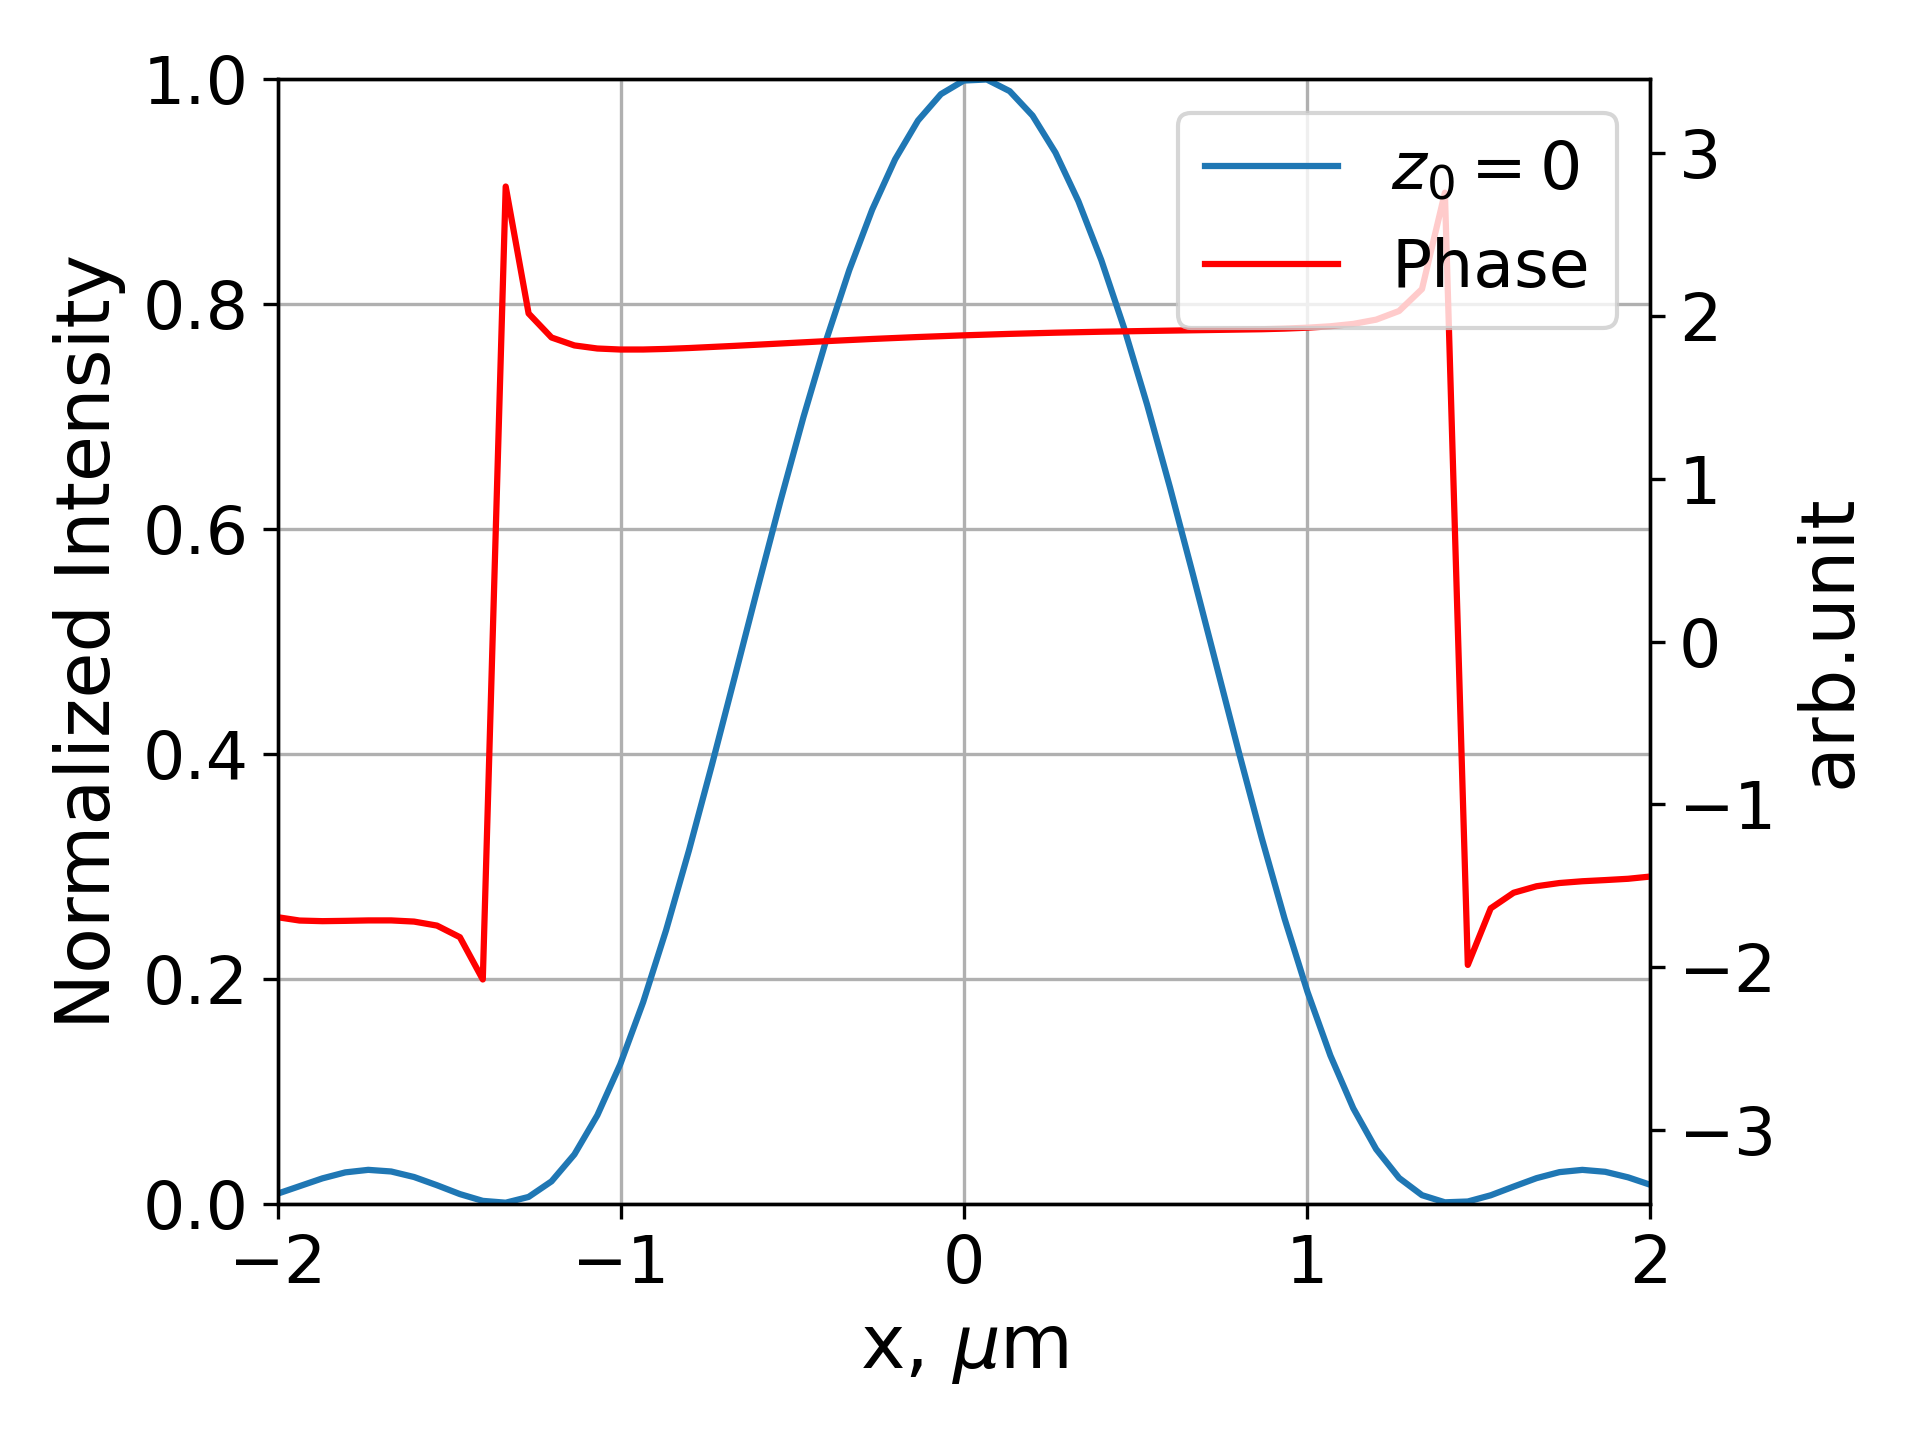
\includegraphics[width=\linewidth]{content/images/Synchrotron_Radiation/intensity_scan_N_w_100_phase_study_cross_middle.png}
            \captionsetup{justification=centering}
            \caption{Imaginary source distribution in the middle of the undulator at resonance.}  % Add your caption here
            \label{Fig:middle_scan}  % Unique label for referencing
        \end{minipage}
        \hfill  % Adds horizontal space between the figures
        \begin{minipage}{0.48\linewidth}
            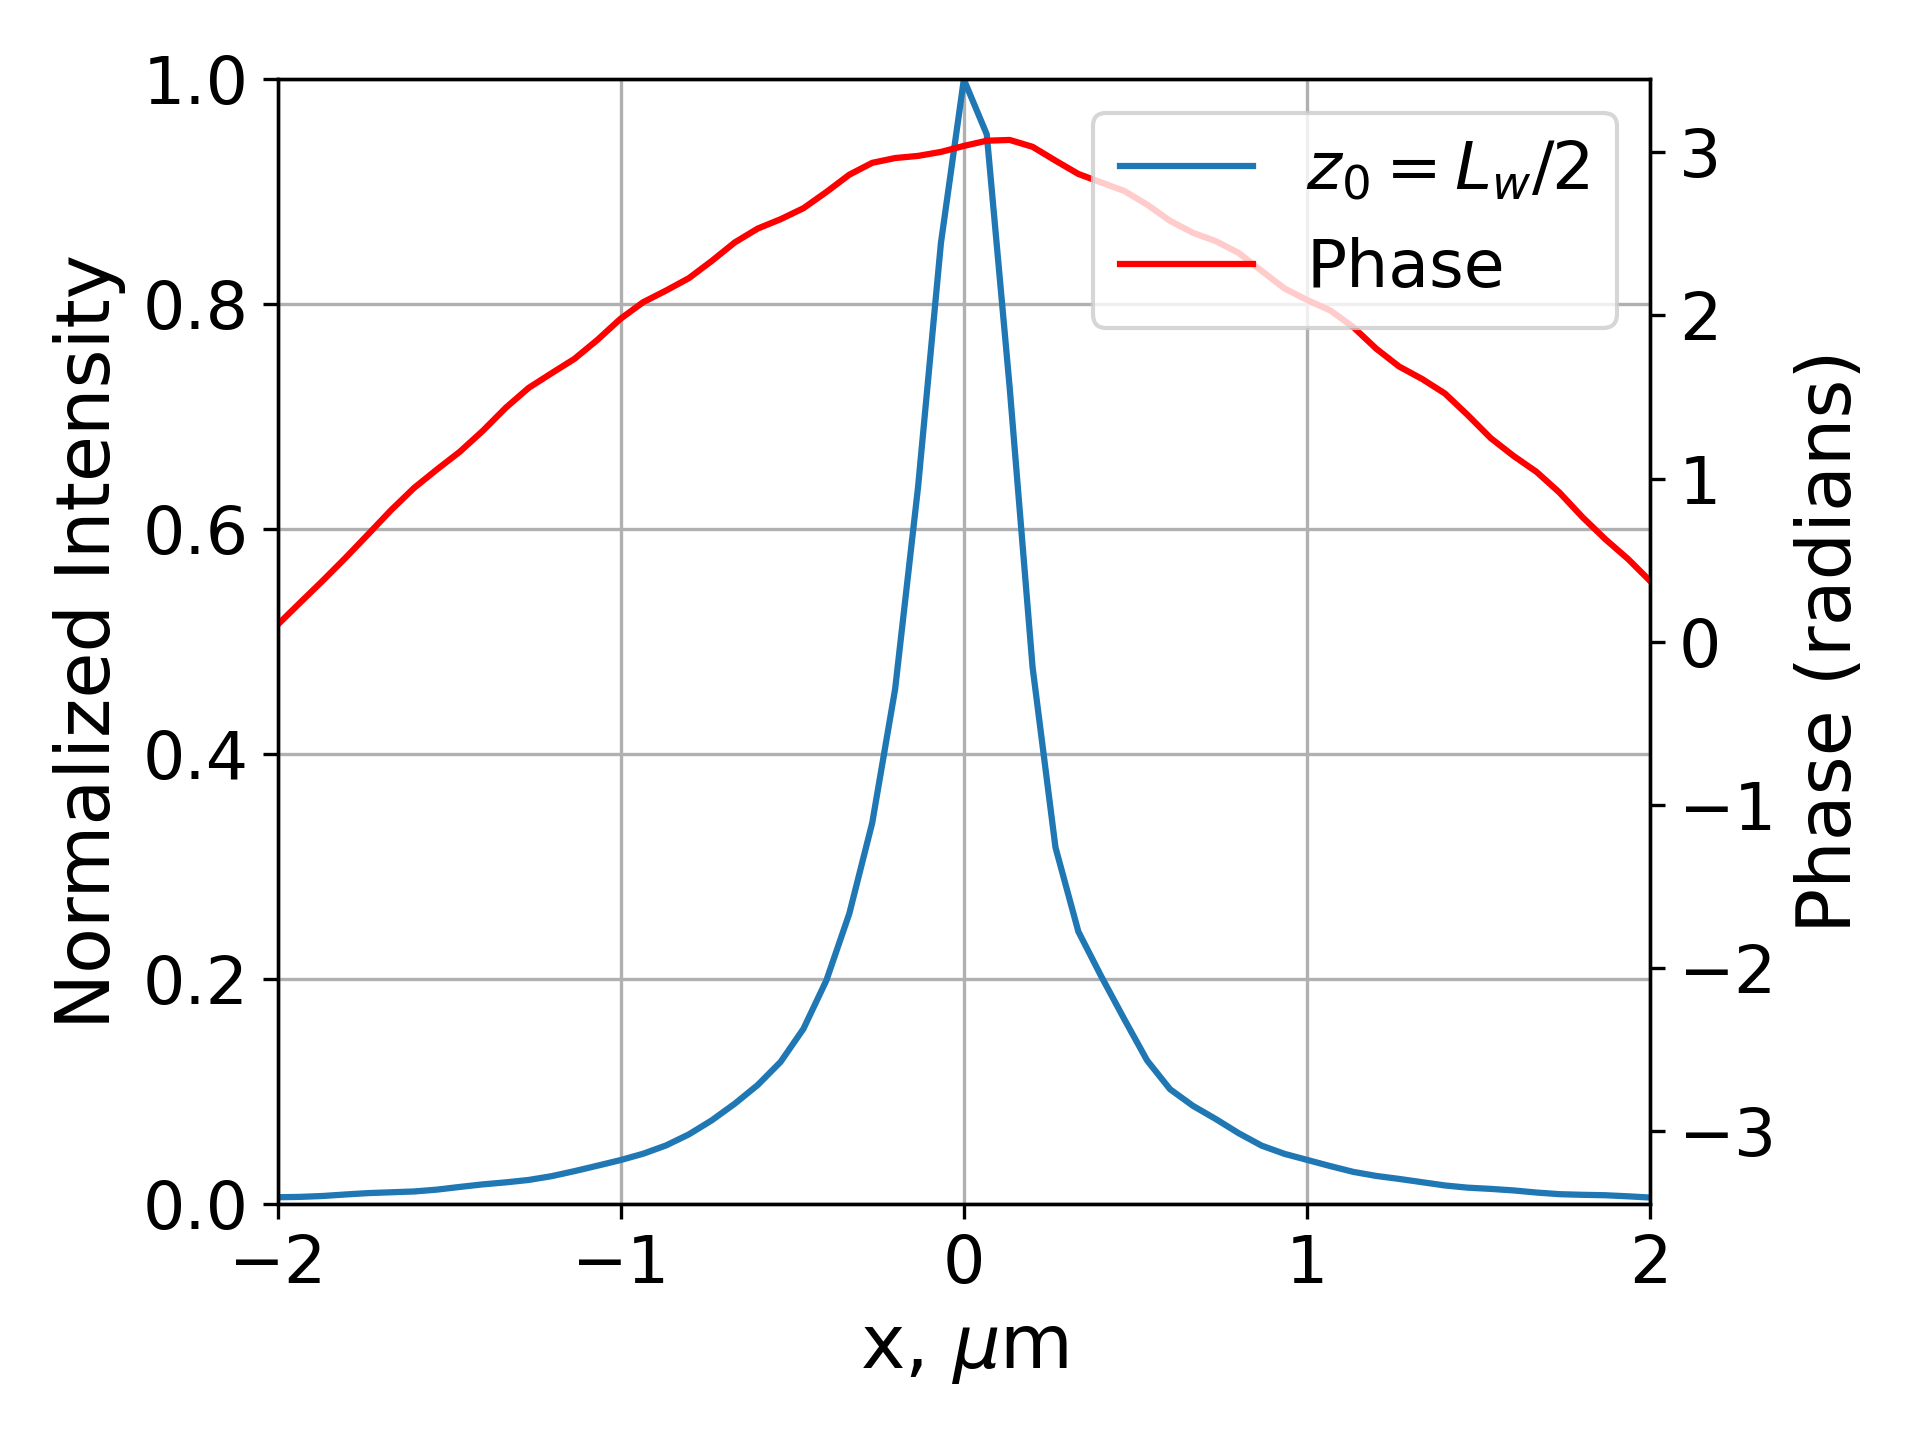
\includegraphics[width=\linewidth]{content/images/Synchrotron_Radiation/intensity_scan_N_w_100_phase_study_cross_end.png}
            \captionsetup{justification=centering}
            \caption{Imaginary source distribution at the edge of the undulator at resonance.}  % Add your caption here
            \label{Fig:end_scan}  % Unique label for referencing
        \end{minipage}
    \end{figure*}        

    Upon free-space propagation, the Wigner function distribution stretches accordingly~\cite{bazarov_synchrotron_2012}, resulting in the types of distributions depicted in the upper subplots of Fig.\ref{Fig:Lw2_wig} at both ends of the undulator. It can be observed that one axis of the "cross" is now oriented parallel to the inverse space axis. A detailed calculation of the spatial distribution reveals that there is no singularity, but the distribution is noticeably narrower compared to the center of the device. For a comparison, see Fig.\ref{Fig:end_scan} and Fig.~\ref{Fig:middle_scan}.
    
    From a mathematical perspective, the singularity arises from the combined application of the resonance approximation and the paraxial approximation, neglecting higher-order contributions in the integrand expansion, as presented in~\cite{geloni_paraxial_2005}. The authors of~\cite{geloni_fourier_2007} note that the far-field distribution and the distribution at the source are related via a Fourier transform (apart from the phase factor), implying that small features at the source correspond to large features in the far zone (and vice versa). However, the resonance and paraxial approximations restrict us to angles in the far zone that are comparable to the size of the central cone of the undulator radiation. For large angles, these approximations fail, and thus, the singularity is not truly singular but has a finite width.
    
    The reasoning presented above provides only a qualitative understanding of the nature of this feature. A reasonable question may be: what would be the size of the radiation observed in Fig.~\ref{Fig:end_scan} in terms of source parameters? Here I mean the following: the undulator radiation diffraction size is $\sqrt{L_w \lambdabar}$, which is related to the physical length of the undulator. This is precisely a resonance effect when all periods contribute to the radiation formation constructively. However, there is another typical scale in the undulator: its period length $\lambda_w$ and a diffraction size associated with $\sqrt{\lambda_w \lambdabar}$, which should also be present in the structure of the undulator radiation. From this point on, I will refer to the diffraction size related to the overall length of the undulator as the resonance one, and the one related to the undulator's period as the non-resonance one.
    
\subsection{Undulator source wiggling or out of resonance source distribution}

    To observe the non-resonant diffraction size of undulator radiation, two methods can be employed: decreasing the number of undulator periods or observing the radiation out of resonance. The first approach mitigates the resonance effect of the device. The flux density intensity scales proportionally to the square of the number of undulator periods. Thus, by reducing the number of undulator periods, one can observe more intrinsic details of the radiation at the source, which are not obscured by the resonance diffraction size. The second approach, observing radiation out of resonance, removes any resonance effects, allowing for the observation of the pure non-resonant diffraction size. I expect this size to significantly differ from the well-known resonant diffraction size: $\sqrt{L_w \lambdabar}$.
    
    If I attempt to show it mathematically I start with the far zone expression of the electric field. Modifying Eq.~\ref{Eq:funal_Eq_for_SR}: expanding $1/(z_0 - z')$ around $z_0$ and using $\vec{\theta} = (\vec{r}_{\perp_0} - \vec{r}'_{\perp}) / (z_0 - z')$ I write:
    \begin{align}
        \vec{\tilde{E}}(\vec{\theta}, z_0, \omega) = -\frac{i \omega e}{c^2 z_0} \int_{-\infty}^{\infty} dz' \left( \frac{\vec{v}(z')}{c} - \vec{\theta} \right) \exp\left( i \omega \left[ \frac{s(z')}{v} - \frac{z'}{c} \right] + \frac{i \omega}{2 c} \left[ z_0 \theta^2 - 2 \vec{\theta} \cdot \vec{r}'(z') + z' \theta^2 \right] \right)
        \label{Eq:far_zone_field_wiggling_feature}
    \end{align}
    I can obtain the virtual source field at the position $z = z_s$ from Eq.~\ref{Eq:far_zone_field_wiggling_feature} by back propagating this field to the source location using the expression from~\cite{geloni_fourier_2007}:
    \begin{align}
        \vec{\tilde{E}}(\vec{r}, z_s, \omega) = \cfrac{i \omega z_0}{ 2 \pi c}\int_{-\infty}^{\infty} d\vec{\theta} \exp{\bigg[-\cfrac{i \omega \theta^2}{2 c} (z_0 + z_s) \bigg]} \vec{\tilde{E}}(\vec{\theta}, z_0, \omega) \exp{\bigg[\cfrac{i \omega}{c}\vec{r}\cdot\vec{\theta} \bigg]}.
    \end{align}
    and substituting Eq.~\ref{Eq:far_zone_field_wiggling_feature} in this I obtain:
    \begin{align}
        \vec{\tilde{E}}(\vec{r}, z_s, \omega) = \cfrac{\omega^2 e}{2 \pi c^3} \int_{-\infty}^{\infty} dz' \int_{-\infty}^{\infty} d\vec{\theta} \left( \frac{\vec{v}(z')}{c} - \vec{\theta} \right) \exp\left( i \omega \left[ \frac{s(z')}{v} - \frac{z'}{c} \right]\right) \cr \exp\left(\frac{i \omega}{2 c} \left[(z' - z_s)\theta^2 + 2\vec{\theta}\cdot (\vec{r} - \vec{r}'(z')) \right] \right).
    \end{align}   
    The first exponent is oscillatory at scales larger than the formation length $L_f$ as one integrates along $z'$. Consequently, the integral limits can be set to $(-L_f, L_f)$ at most. This simplification remains general and does not depend on the type of source considered. The value of $L_f$ can vary significantly depending on the chosen magnetic configuration. For undulator radiation, I seek evidence that the diffraction size differs from the resonant one determined by the length of the undulator $L_w$.

    The second exponent contains a phase that is also oscillatory as one integrates over $\vec{\theta}$. Intuitively, within the range of $z_s$ around the "virtual source" ($-L_f, L_f$), the integral is significant for $\vec{r} \approx \vec{r}'(z_s)$. According to the energy conservation law, all energy in the pulse will be concentrated around this location at the source.
    
    Thus, I estimate the integration range for angles to be $\theta_{x, y} < \sqrt{2c/(\omega (z' - z_s))}$, assuming $z'$ varies only slightly within ($-L_f, L_f$). We observe large field values only within ($-L_f, L_f$) since the field diverges further from the source. Therefore, at most $|z' - z_s| \sim L_f$, giving the estimation $\theta_{x, y} < \sqrt{2c/(\omega L_f)}$. Finally, the last term remains small only for deviations of $\vec{r}$ from the trajectory up to the order of $\delta r \sim c / \omega \sqrt{\omega L_f / c} \sim \sqrt{(cL_f)/\omega}$, which is the typical diffraction size.

    At this point, I have determined that the diffraction size of the radiation is $\delta r \sim \sqrt{(cL_f)/\omega}$, as expected. It does not contradicts the hypothesis that there are two typical scales: one related to the undulator length and the other to its period length. The former is usually associated with undulators, where the diffraction size is considered to be $\sqrt{(cL_w)/\omega}$. However, the presence of the second natural scale suggests that there should be a smaller diffraction size related to the device period $\lambda_w$, thus the diffraction size can be written as $\sqrt{(c\lambda_w)/\omega}$. 
    
    To confirm this hypothesis, I shall break the resonance approximation typically used in analytical calculations and decrease the number of undulator periods. This results in a specific "wiggling" of the undulator source, as illustrated in Figs.~\ref{Fig:intensity20}, \ref{Fig:intensity10}, \ref{Fig:intensity5}. 
    \begin{figure*}[p] 
        \centering
        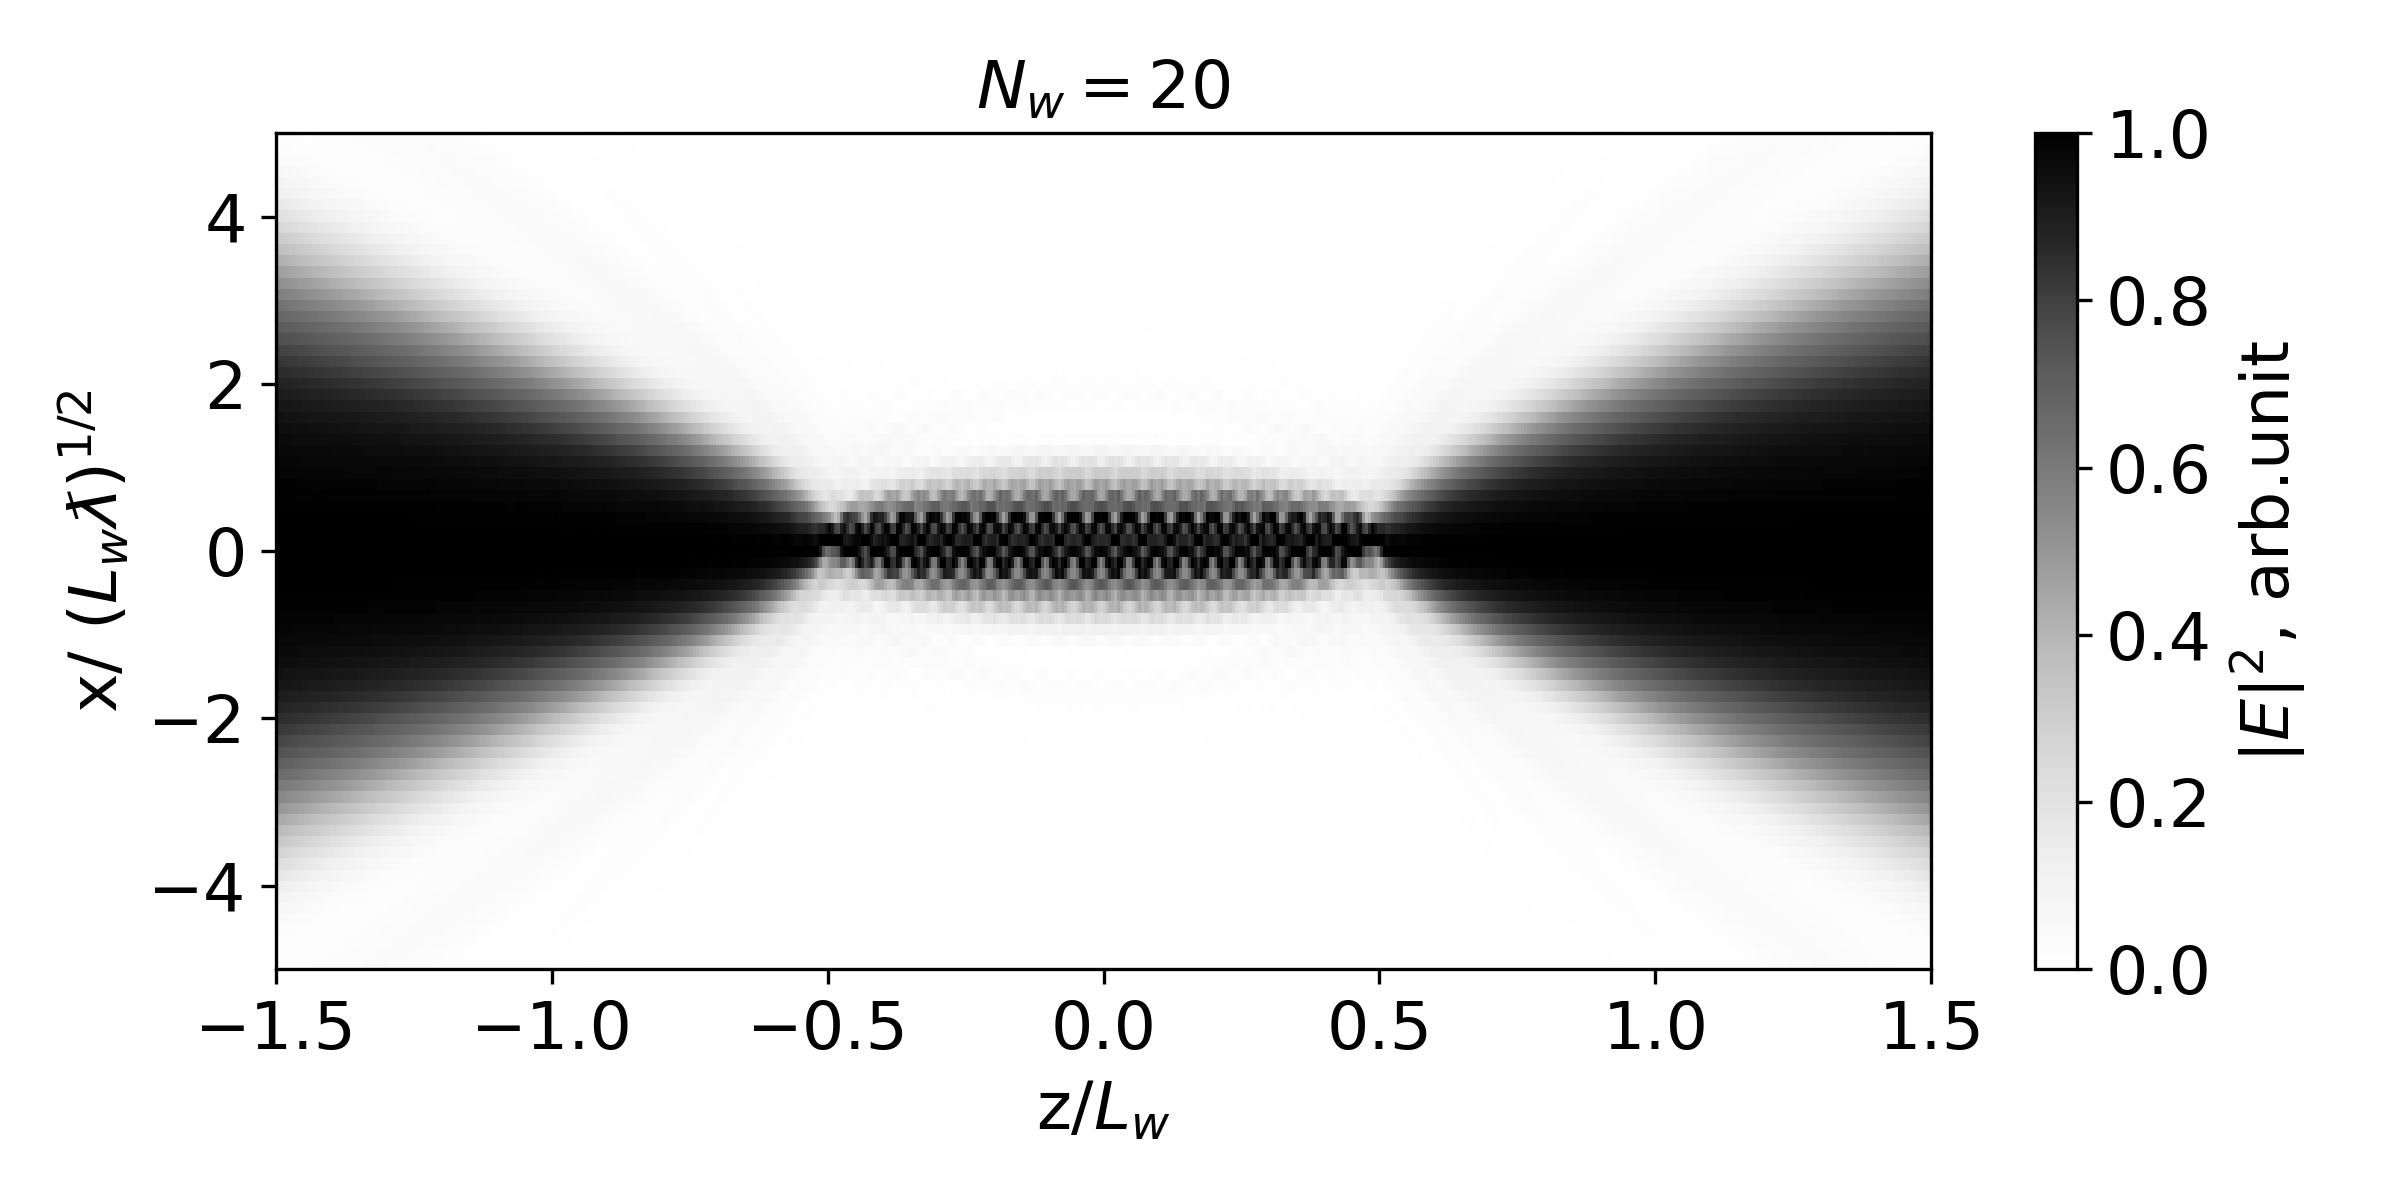
\includegraphics[width=0.9\linewidth]{content/images/Synchrotron_Radiation/intensity_scan_N_w_20.png}
        \captionsetup{justification=centering}
        \caption{}
        \label{Fig:intensity20}
        
        \vspace{\floatsep} % Adds some space between the figures
        
        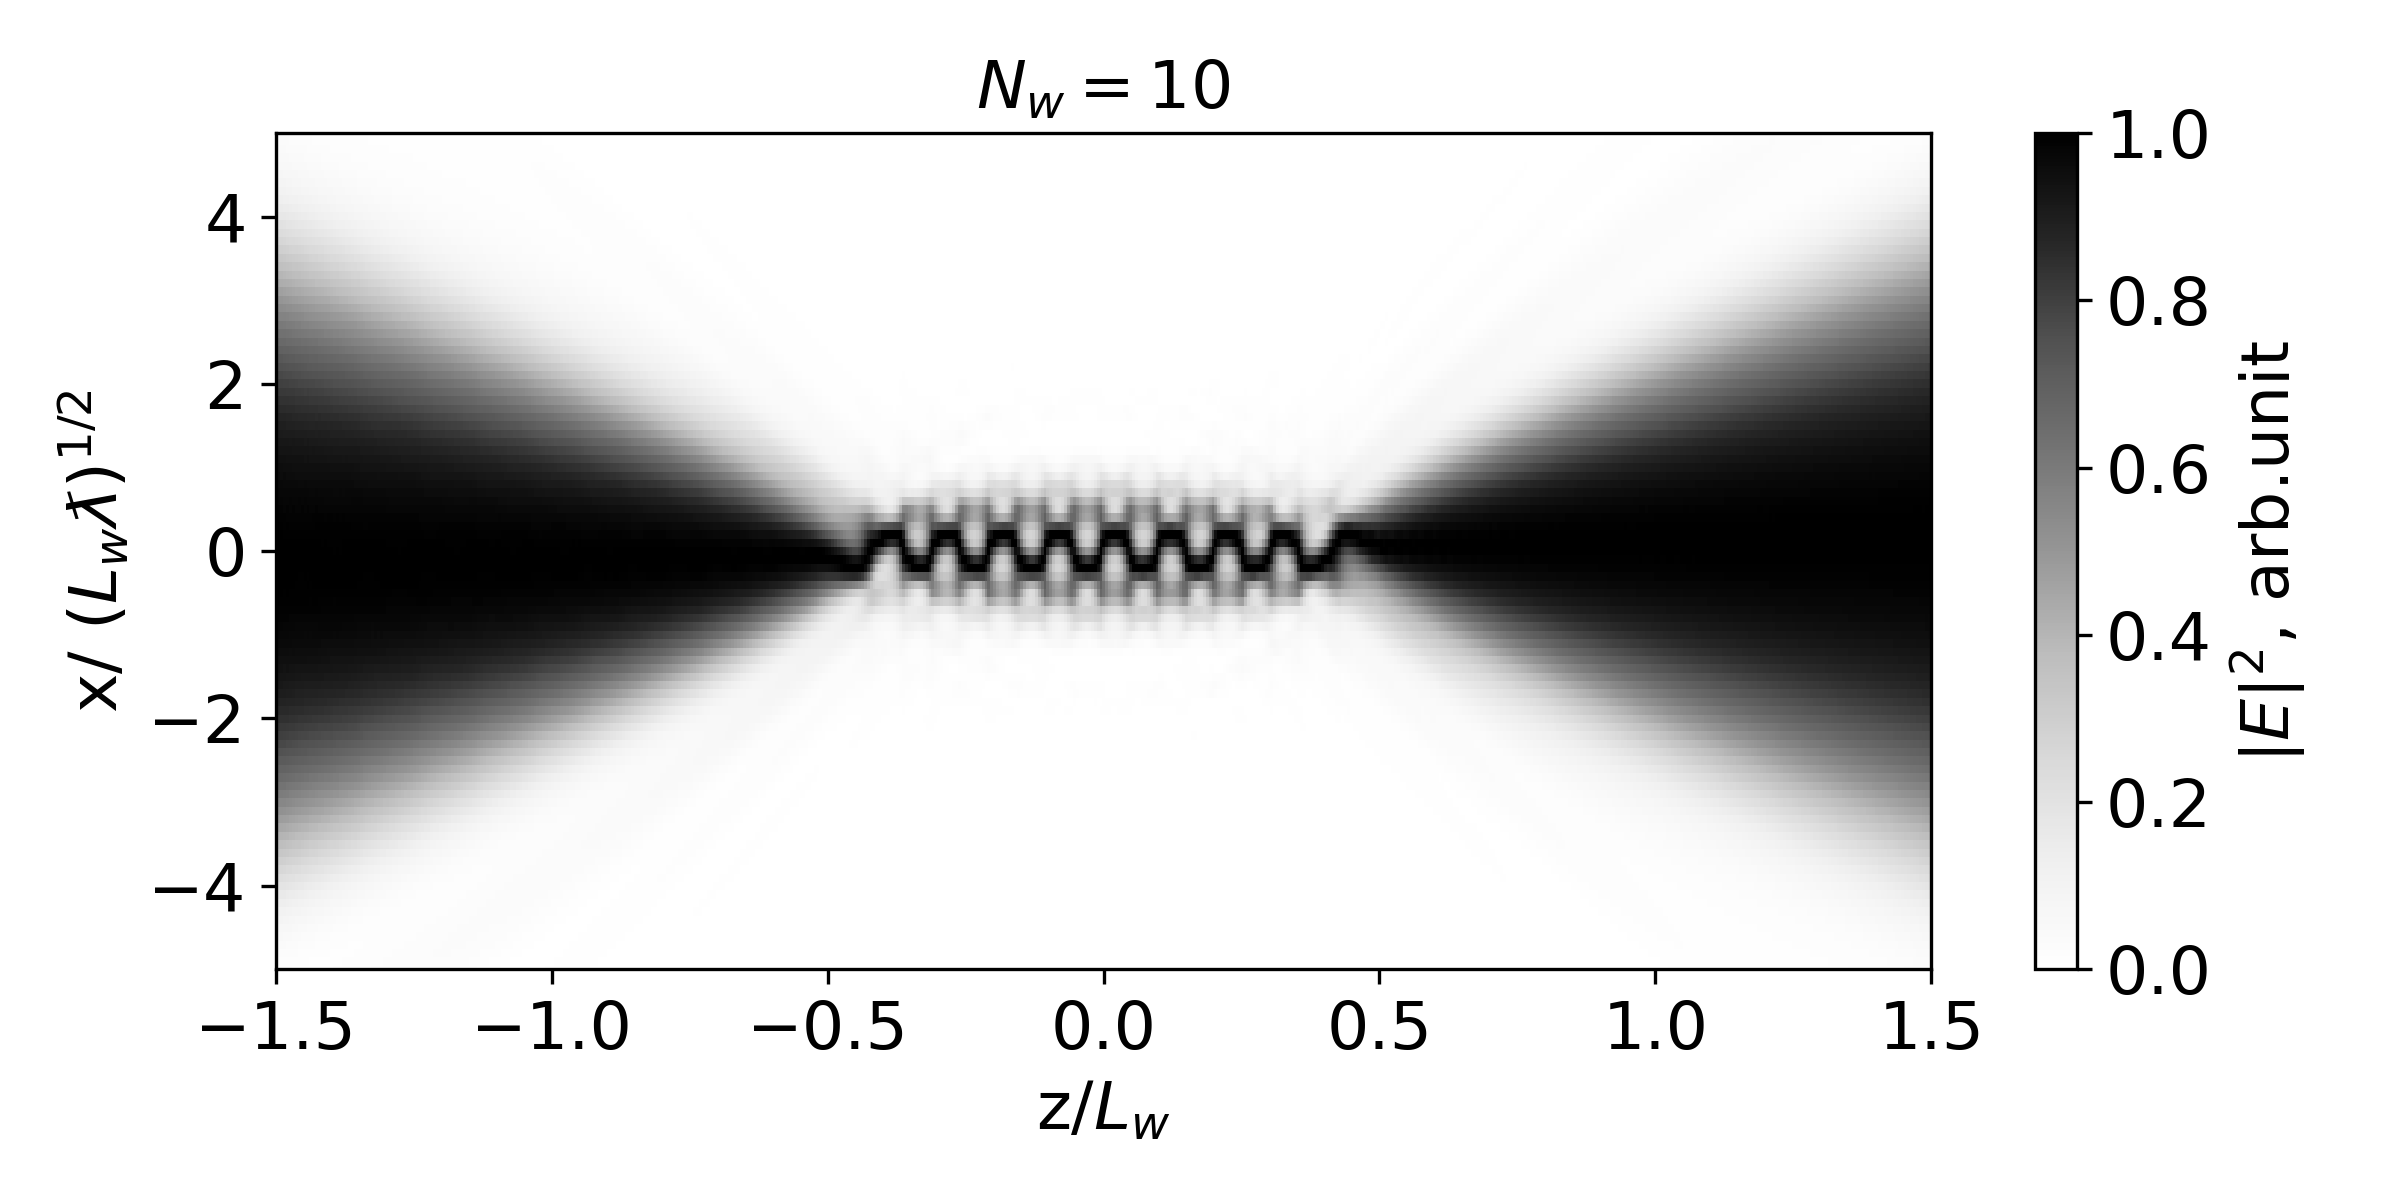
\includegraphics[width=0.9\linewidth]{content/images/Synchrotron_Radiation/intensity_scan_N_w_10.png}
        \captionsetup{justification=centering}
        \caption{}
        \label{Fig:intensity10}
        
        \vspace{\floatsep} % Adds some space between the figures
        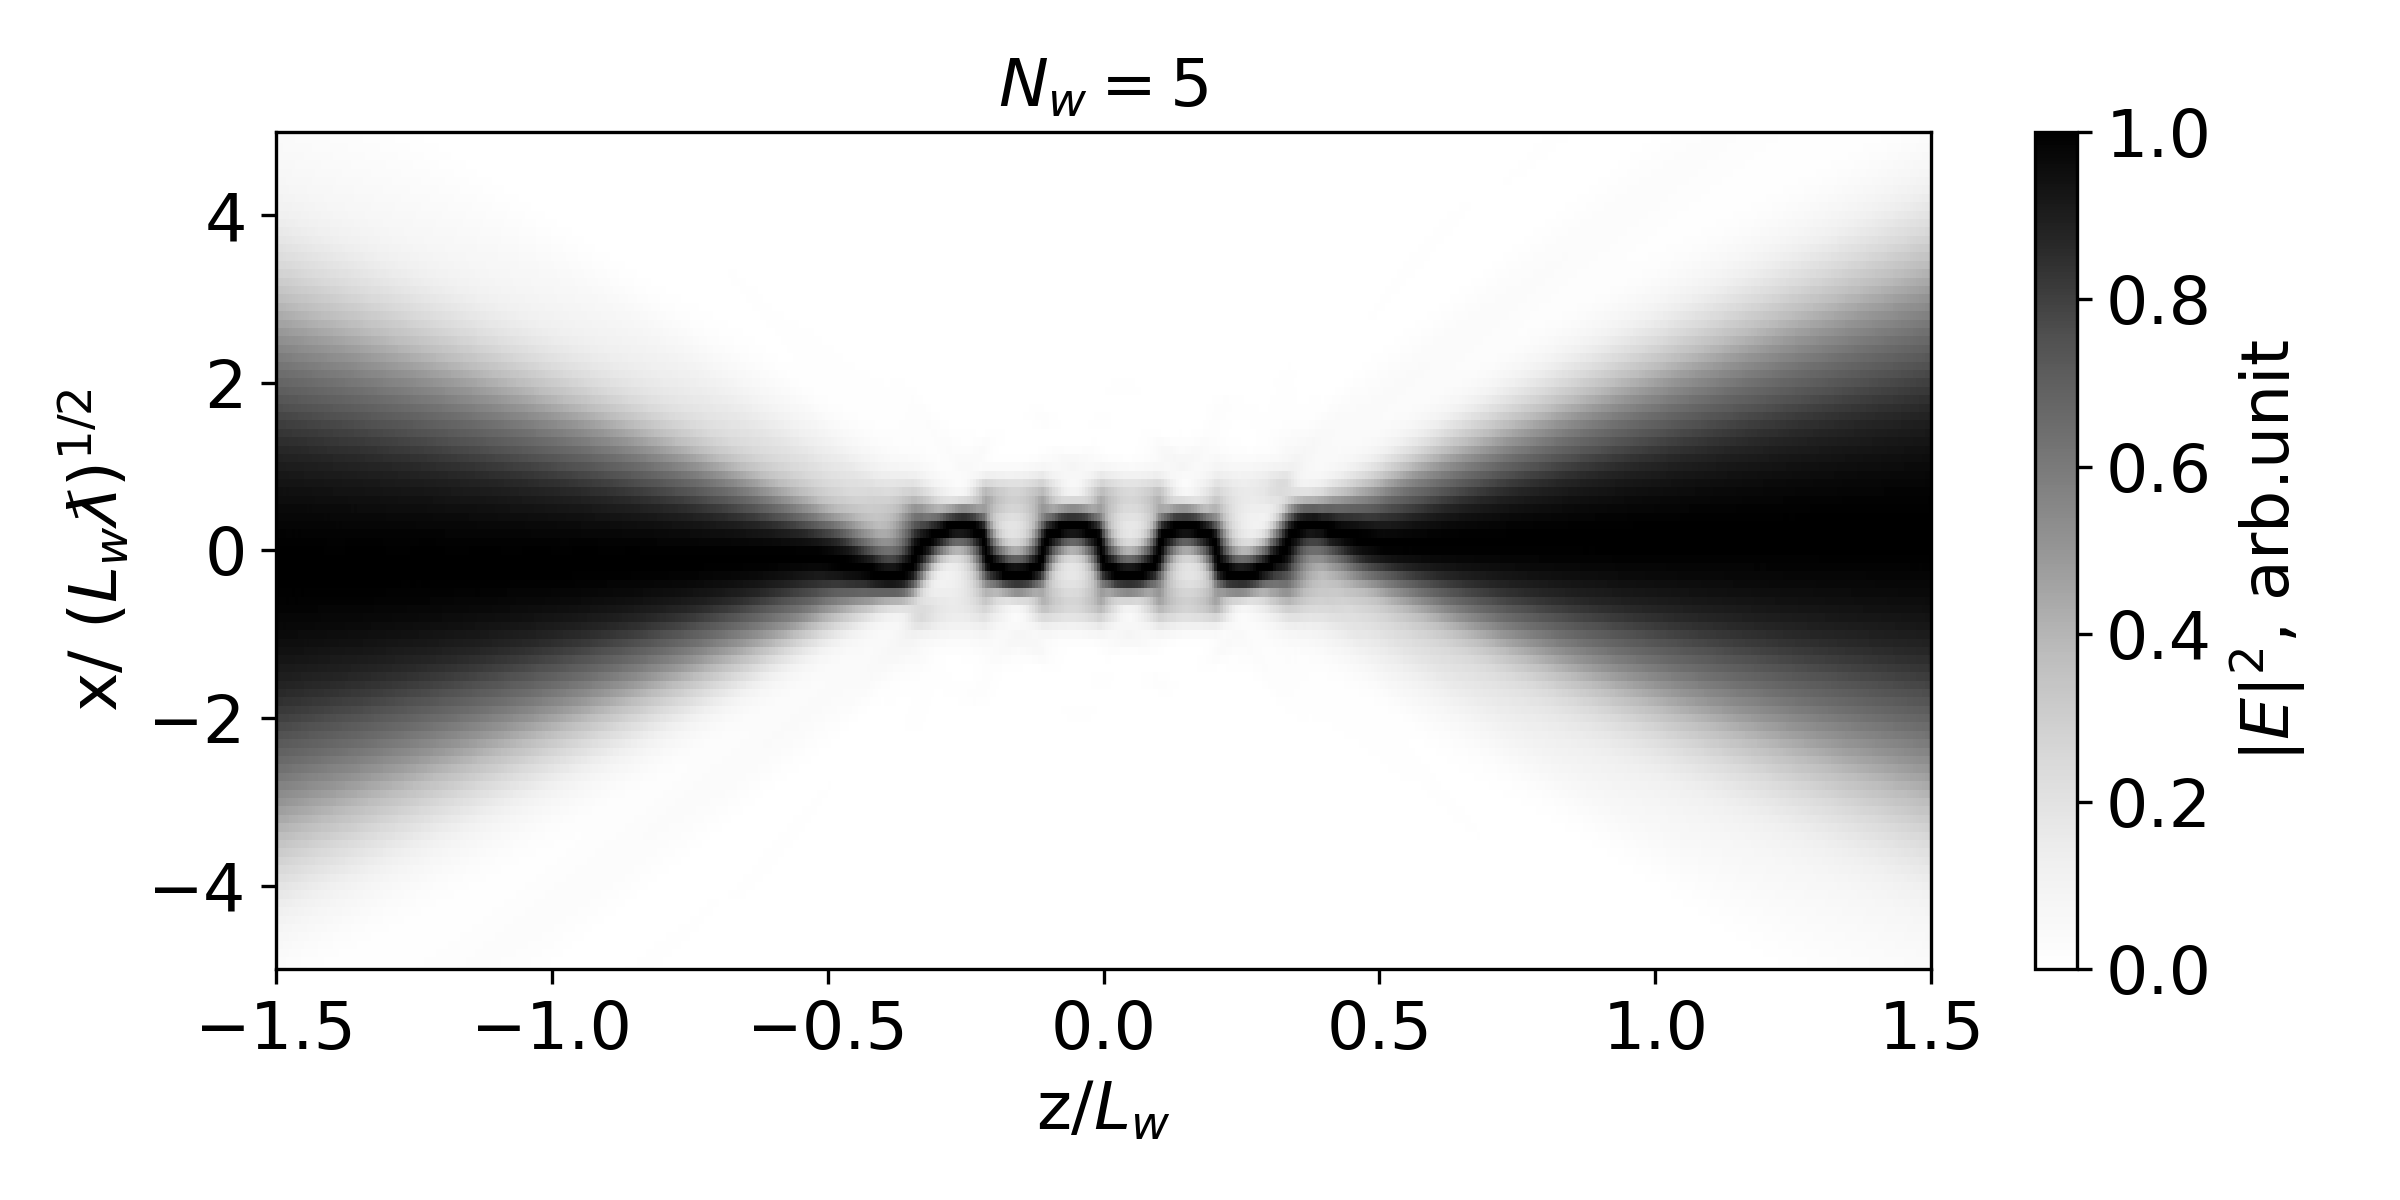
\includegraphics[width=0.9\linewidth]{content/images/Synchrotron_Radiation/intensity_scan_N_w_5.png}
        \captionsetup{justification=centering}
        \caption{"Wiggling" of the undulator source distribution. From up to down source distributions of 20 periods, 10 period, and 5 period devices.}
        \label{Fig:intensity5}
    \end{figure*}
    As one can see, I observe a finer, non-resonant structure of the undulator radiation superposed with the resonant one. 

    To clearly observe this effect, I examine the out-of-resonance case of the same radiation from a ten-period device. One can observe the "pure" wiggling of the source as depicted in Fig.~\ref{Fig:intensity_scan_N_w_10_out_of_resonance}, and intensity slices over specific locations are shown in Fig.~\ref{Fig:intensity_scan_N_w_10_out_of_resonance_slices}.

    \begin{figure*}[h!]
        \centering
        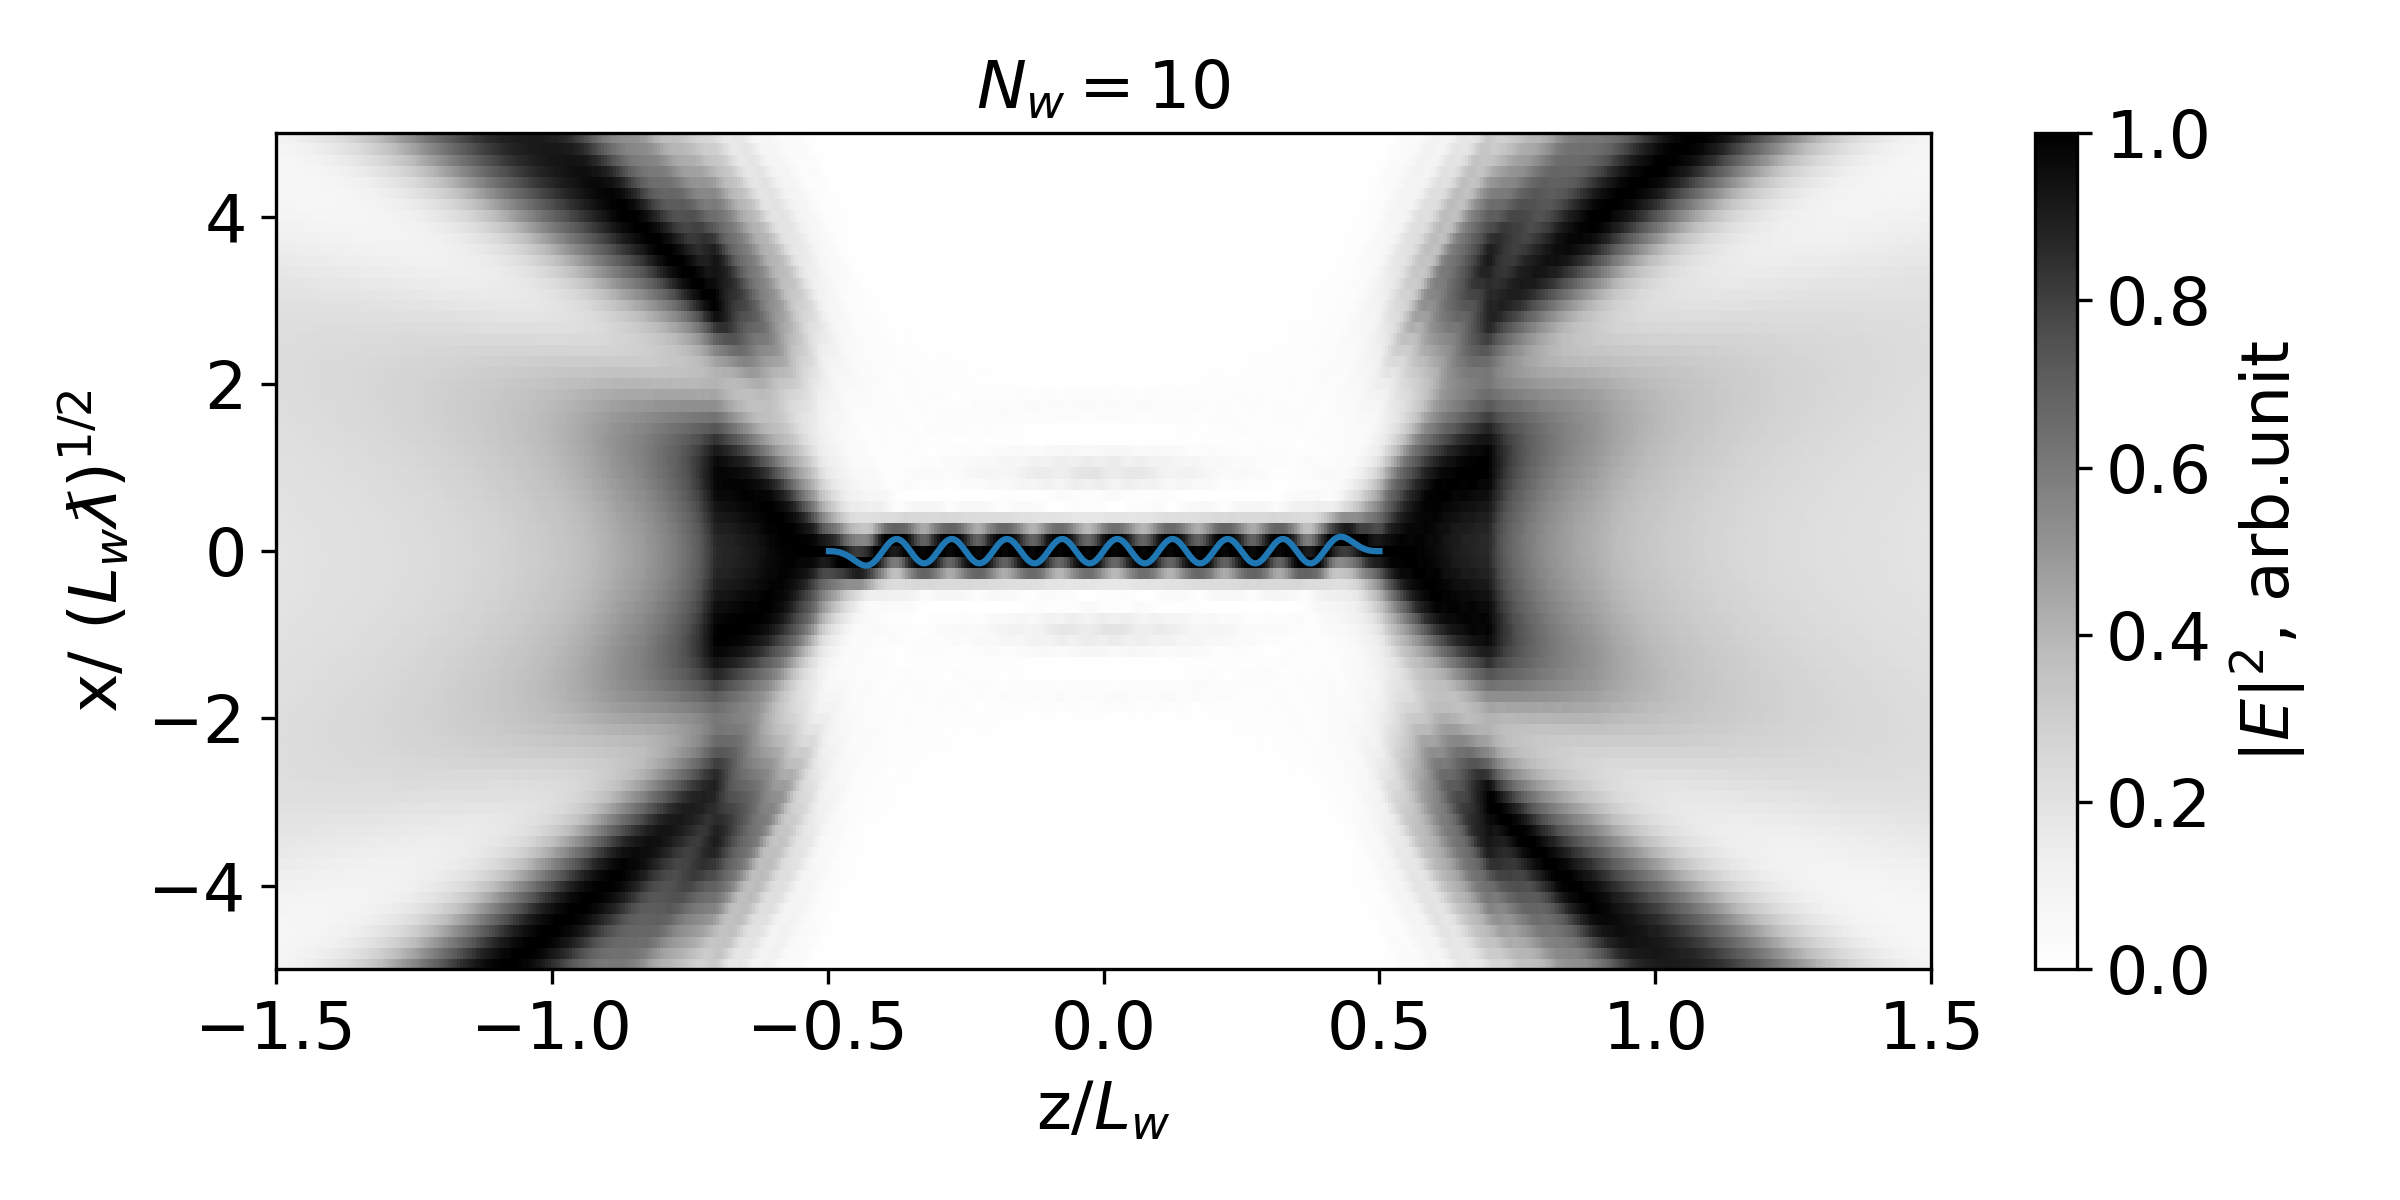
\includegraphics[width=0.9\linewidth]{content/images/Synchrotron_Radiation/intensity_scan_N_w_10_out_of_resonance.png}
        \captionsetup{justification=centering}
        \caption{"Wiggling" of the undulator source distribution for the out-of-resonance case, with the frequency set between the 1st and 2nd harmonics.}
        \label{Fig:intensity_scan_N_w_10_out_of_resonance}
    \end{figure*}

    \begin{figure*}[h!]
        \centering
        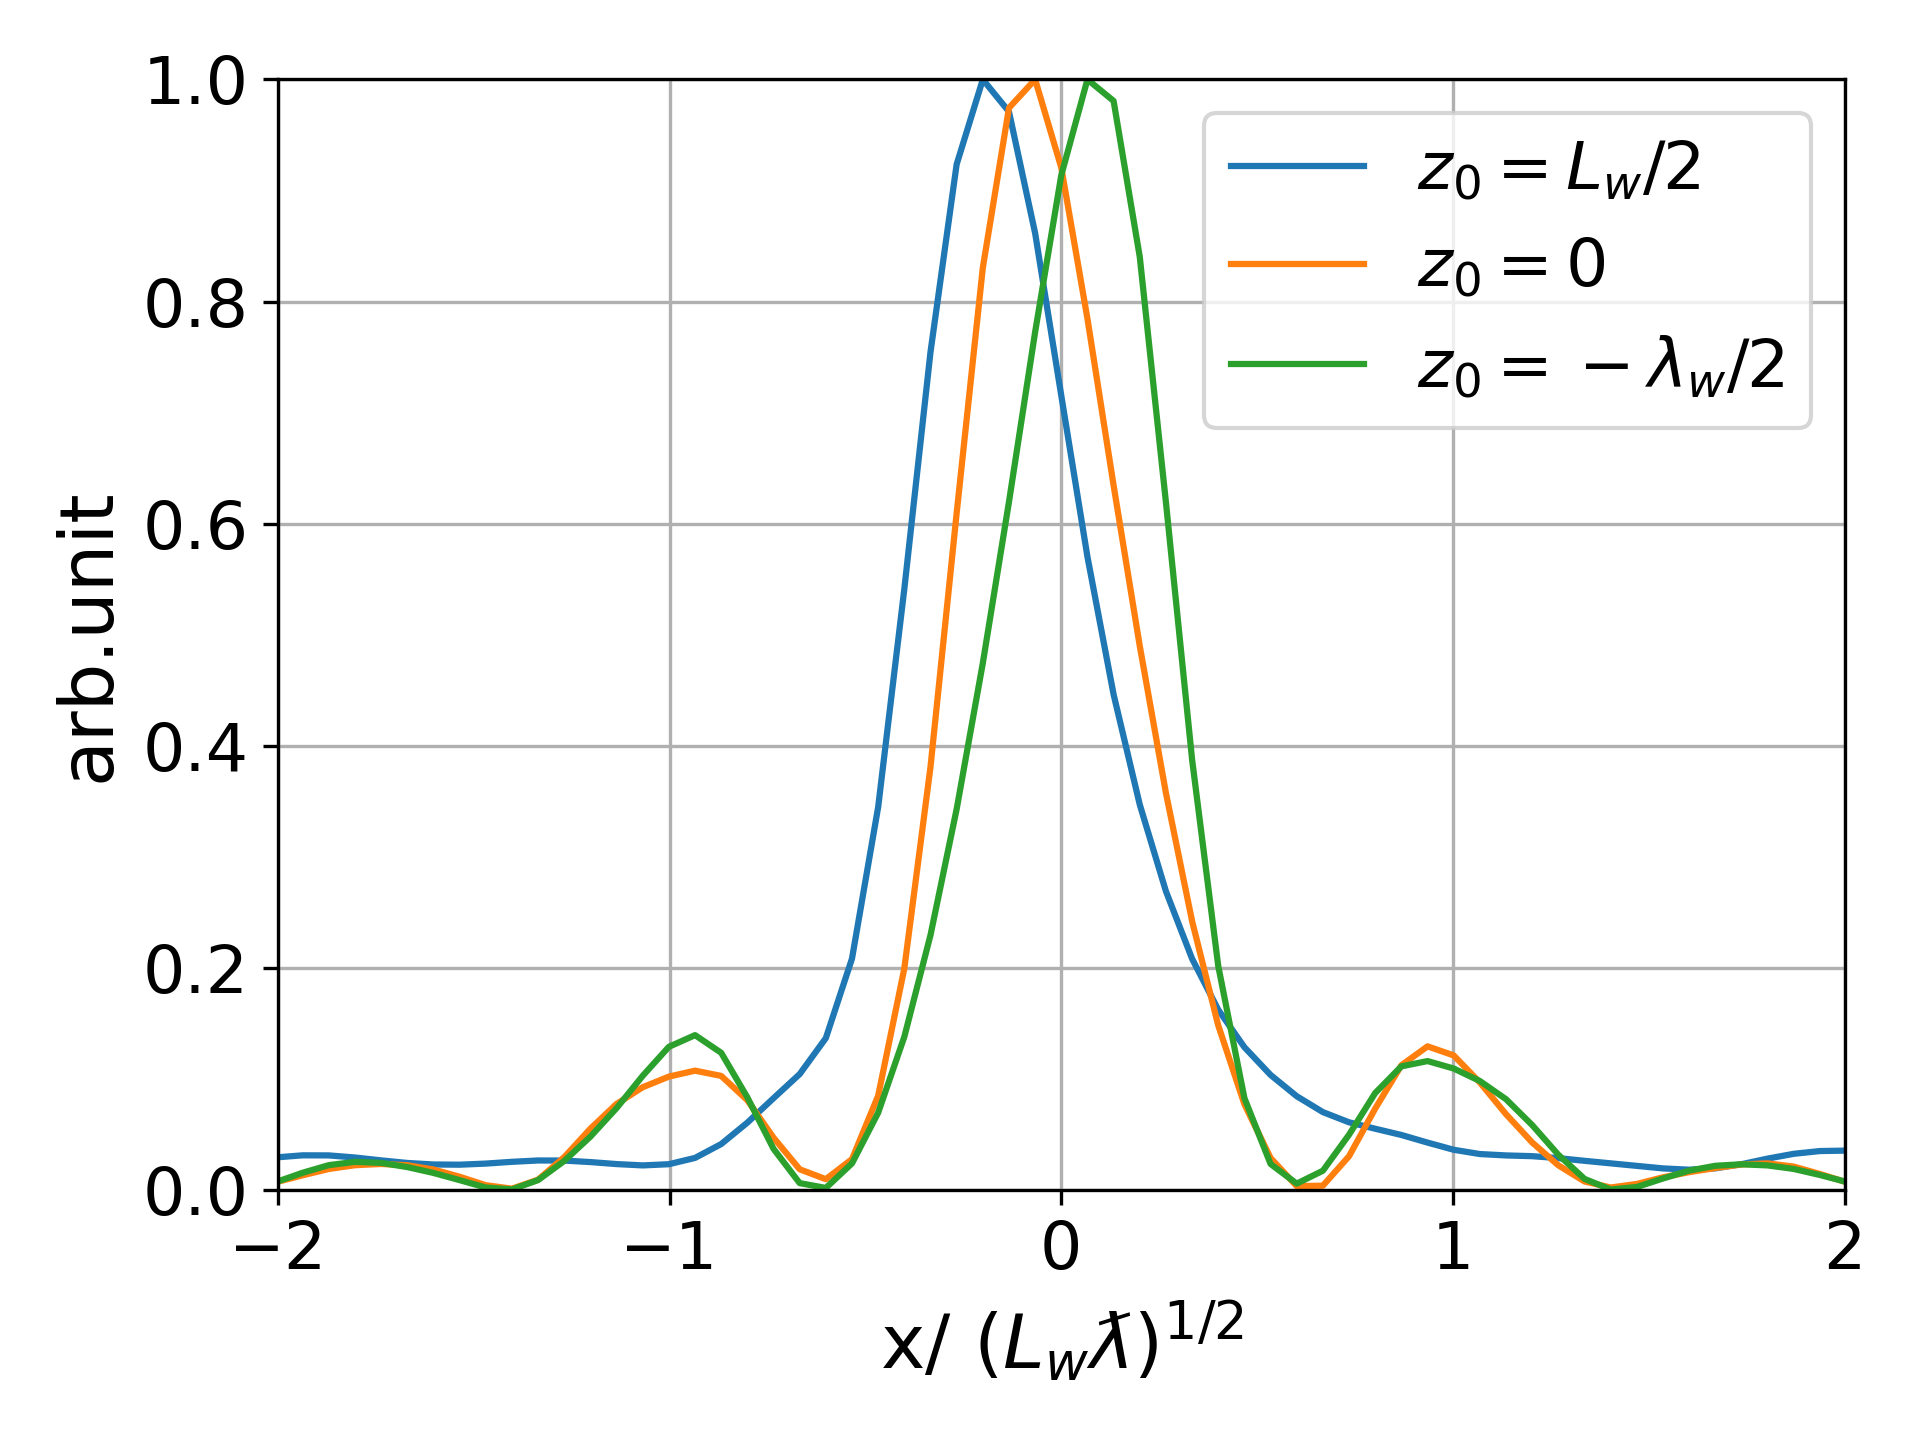
\includegraphics[width=0.5\linewidth]{content/images/Synchrotron_Radiation/intensity_scan_N_w_10_out_of_resonance_slices.png}
        \captionsetup{justification=centering}
        \caption{"Wiggling" of the undulator source distribution for the out-of-resonance case shown for the intensity slices.}
        \label{Fig:intensity_scan_N_w_10_out_of_resonance_slices}
    \end{figure*}
    The most straightforward measurements needed to reveal the non-resonant diffraction size of undulator radiation are coherence measurements of the out-of-resonance undulator radiation. This method reveals the coherence area, the size of which is related to the single-electron radiation diffraction size. In this case, one would expect to detect a significantly smaller coherence area compared to the in-resonance case at the same wavelength. These measurements do not require special conditions, but an interferometers should be placed off the optical axis because the radiation will be observed out of resonance. 
    
    \rr{add citation on possible kinds of interferometers}
    
    The second type of measurement can be direct imaging of the radiation source, provided the emittance of the electron beam is much smaller than the diffraction size of radiation from a single electron. This can be achieved either by using an imaging system with a point spread function much smaller than the single-electron diffraction size or by measuring the wavefront distribution directly \rr{cite} and then using back-propagation methods to trace the radiation back to the source analytically.
    
    \rr{probably, one needs the drawn schemes…}
    
\subsection{Brightness of undulator radiation}
    It is also valuable to examine the brightness of undulator radiation at the source location, defined as the maximum of the Wigner function distribution. This can be achieved by scanning the positions along the undulator and as a function of the detuning parameter $C$ from the resonance, as shown in Fig.~\ref{Fig:badman}.
    \begin{figure*}[h!]
        \centering
        \begin{minipage}[b]{0.48\linewidth}
            \centering
            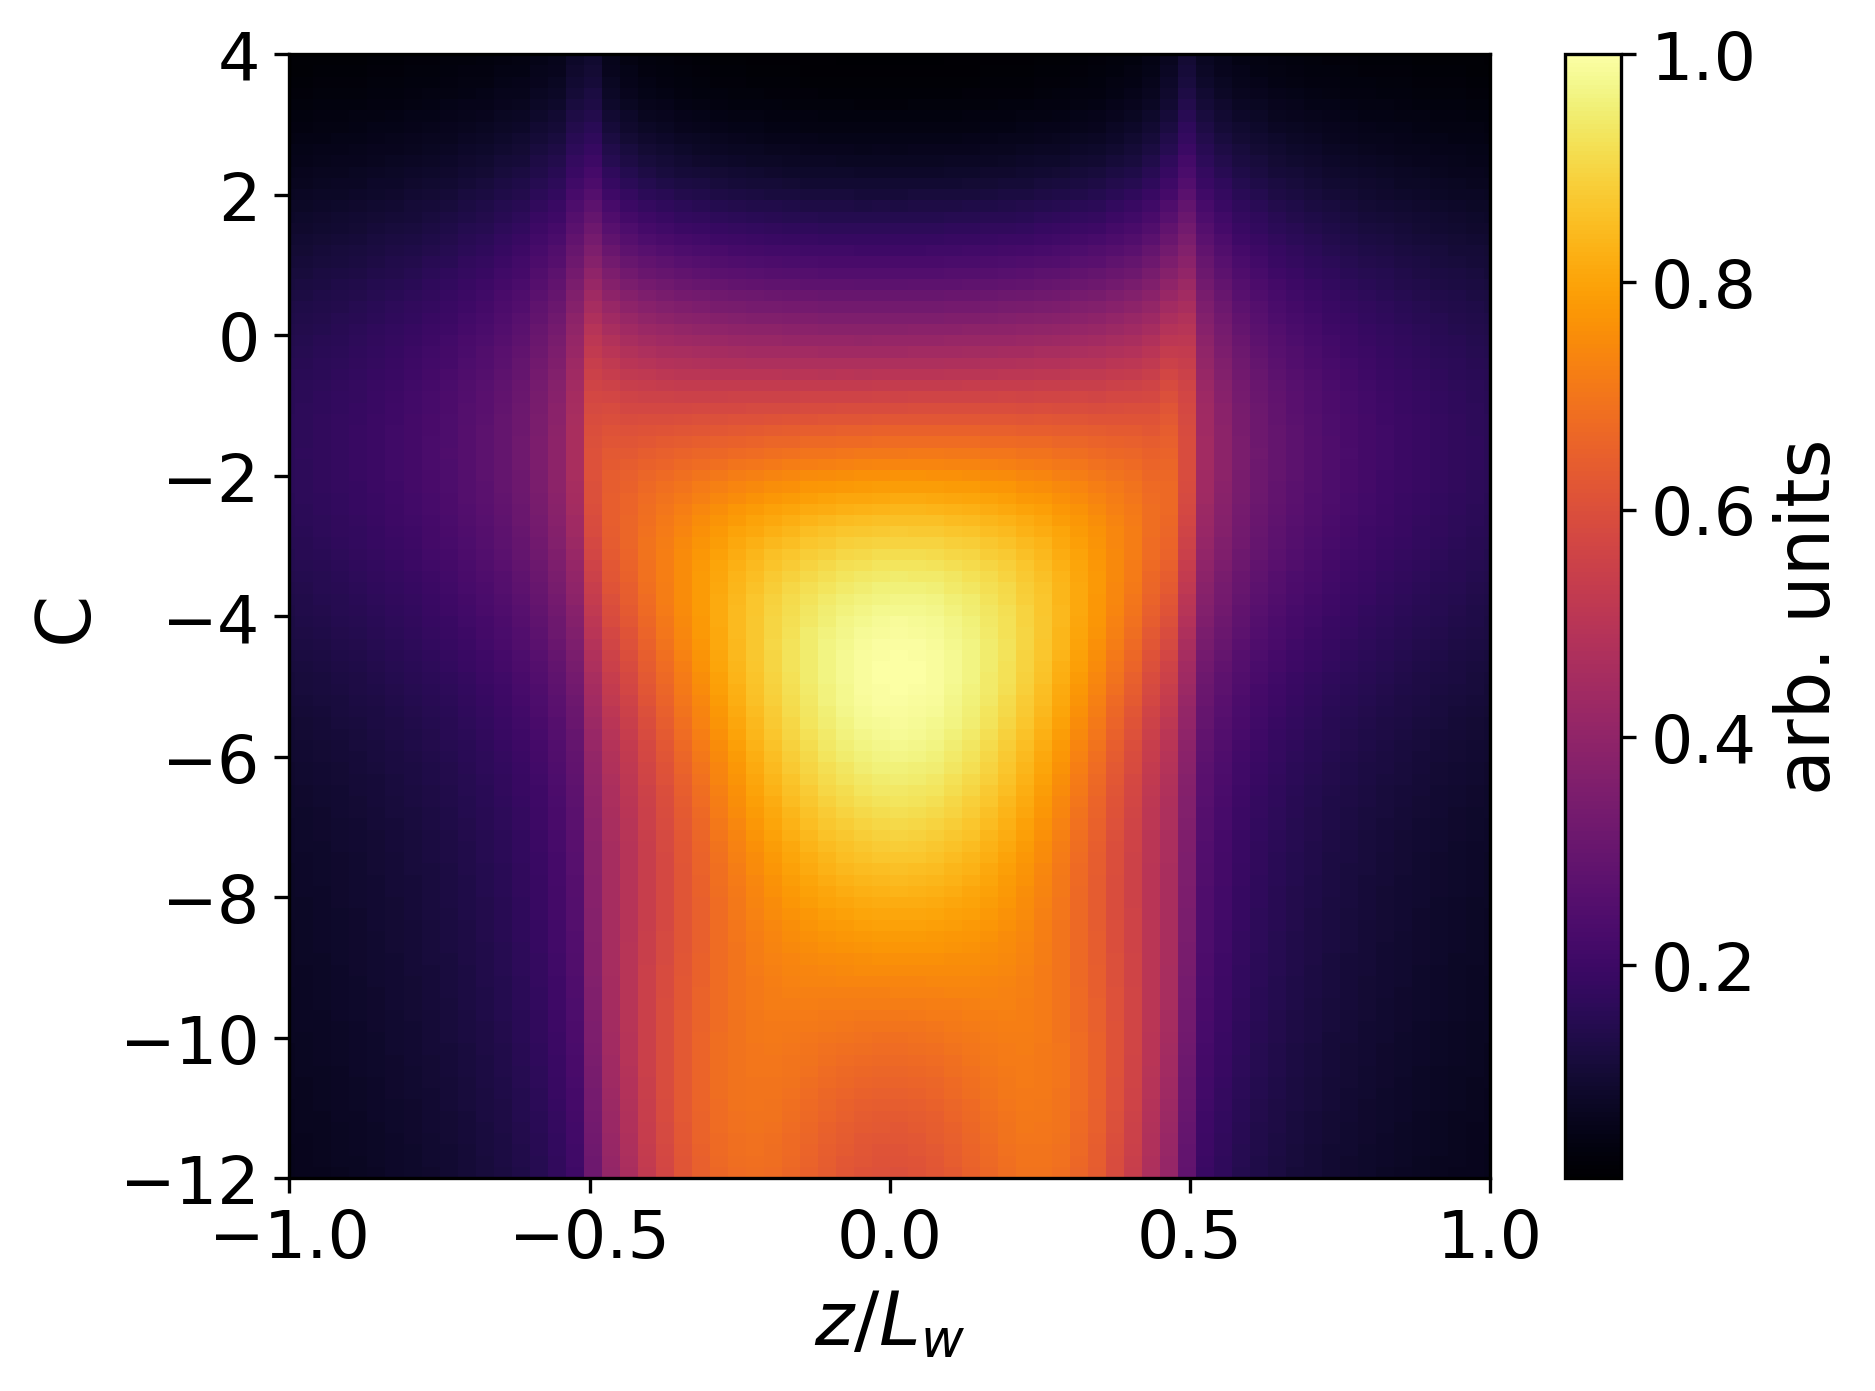
\includegraphics[width=\linewidth]{content/images/Synchrotron_Radiation/badman.png}
            \captionsetup{justification=centering}
            \caption{}
            \label{Fig:badman}
        \end{minipage}
        \hspace{0.02\linewidth}
        \begin{minipage}[b]{0.48\linewidth}
            \centering
            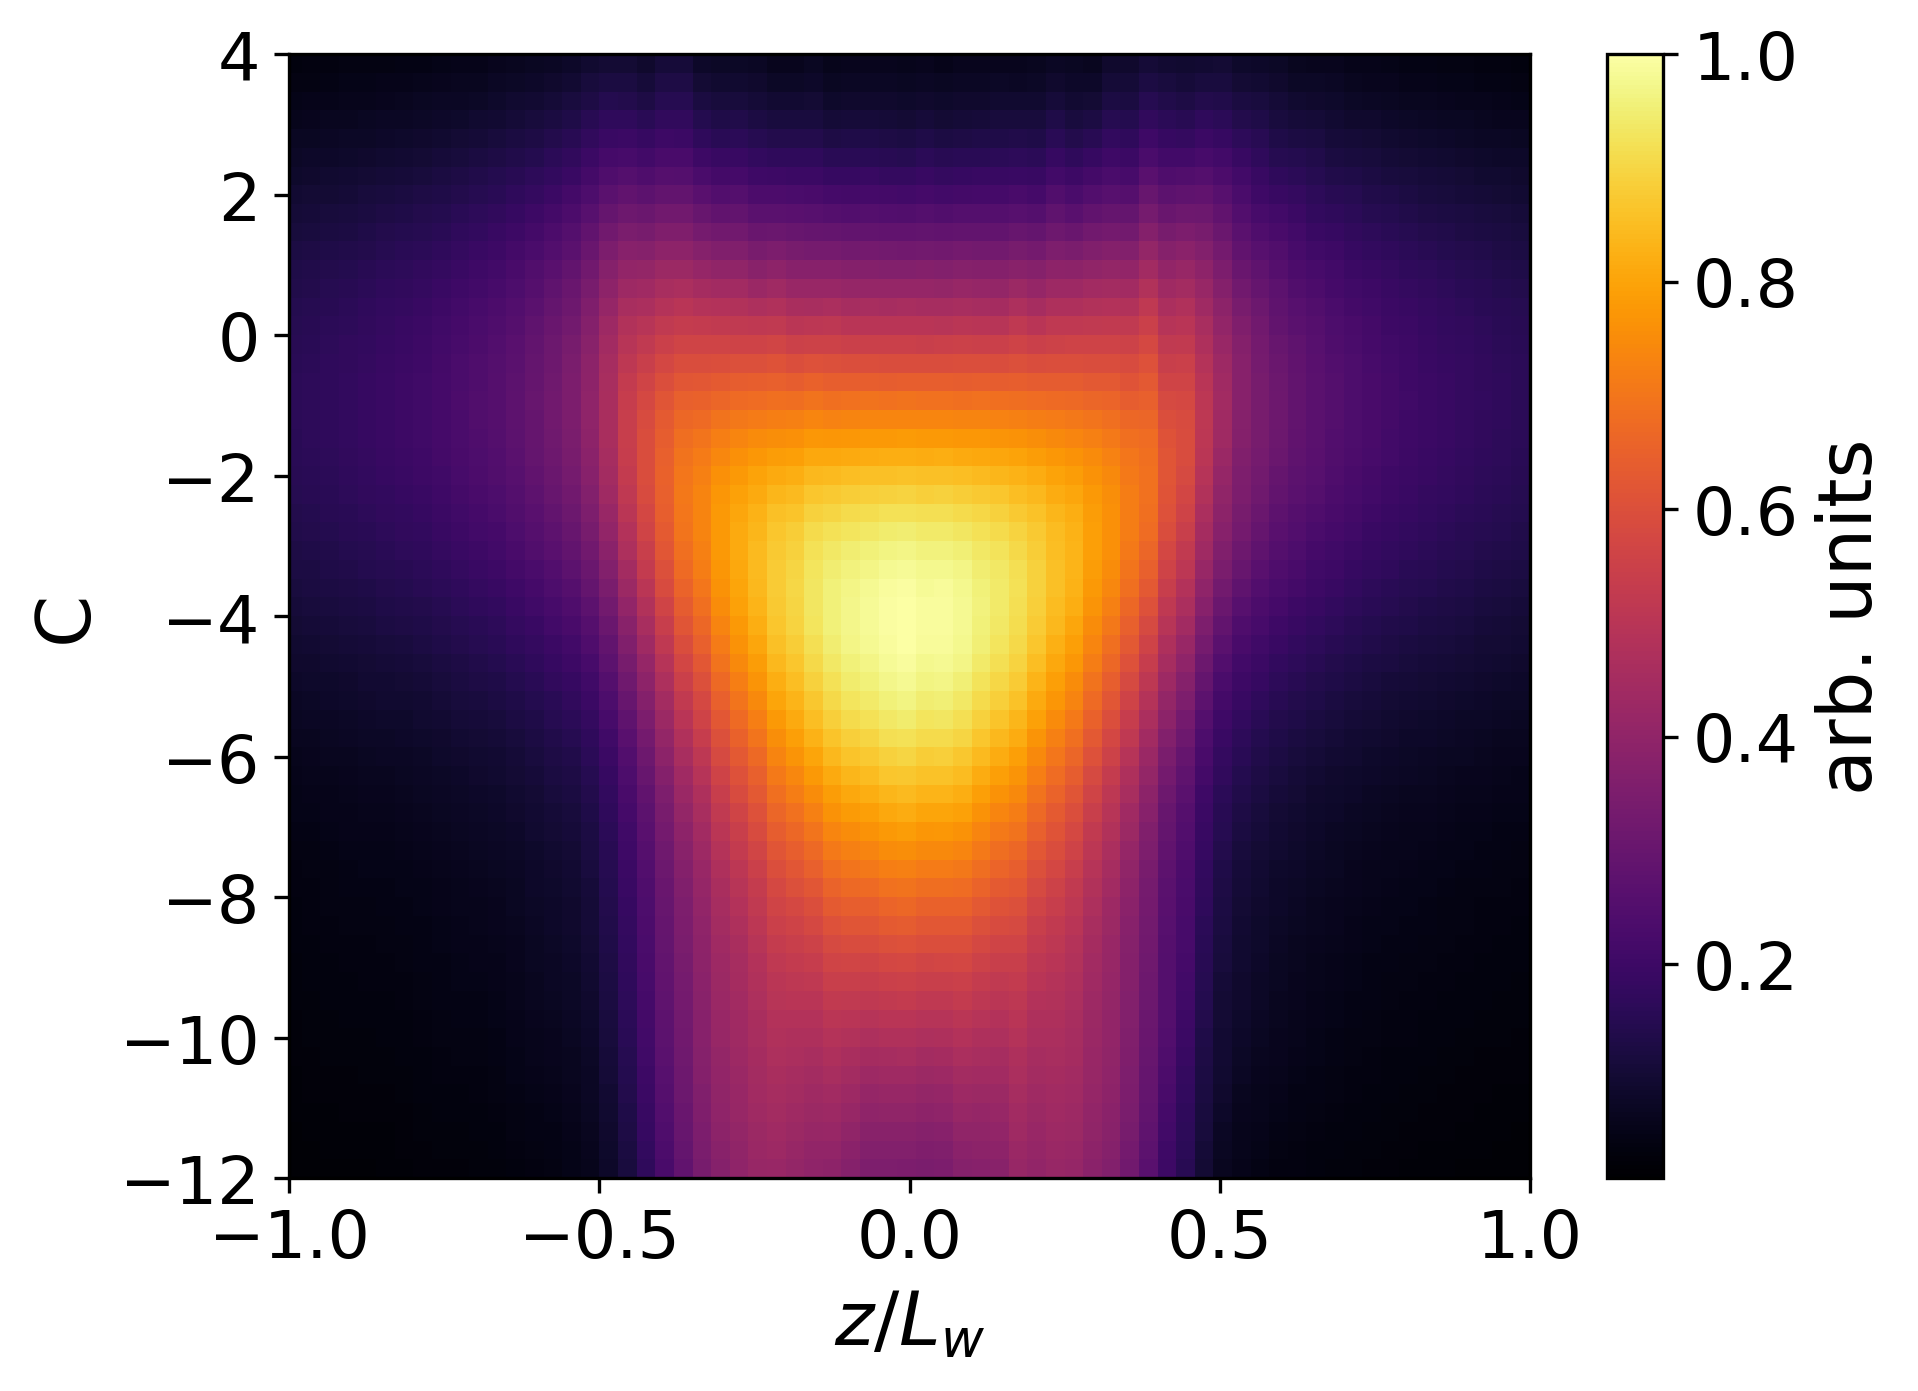
\includegraphics[width=\linewidth]{content/images/Synchrotron_Radiation/badman_Nw_10.png}
            \captionsetup{justification=centering}
            \caption{}
            \label{fig:badman_Nw_10}
        \end{minipage}
        \caption{"Badman" diagram. Horizontal axis corresponds to the position along the undulator and the vertical axis reflects the detuning parameter $C$.}
    \end{figure*}
    Apart from the global maximum around $C = -4$ and $z = 0$, the maxima for the perfectly in-resonance case ($C = 0$) are not located in the middle of the undulator but at either end of the device.

    In conclusion, this effect needs to be studied in more detail both analytically and experimentally. However, an analytical treatment of the problem is complicated when considering undulator radiation not applying the resonance approximation. From the experimental point of view, the measurements does not require subtle setups and can be conducted using the available hardware of modern SR source optical systems only with slight modifications.